\documentclass[12pt, a4paper, titlepage, fleqn]{article}

\usepackage[margin=1in]{geometry}
\usepackage{amsmath}
\usepackage{accents}
\usepackage{etoolbox}
\usepackage{graphicx}
\usepackage{listings}
\usepackage{color} %red, green, blue, yellow, cyan, magenta, black, white
\definecolor{mygreen}{RGB}{28,172,0} % color values Red, Green, Blue
\definecolor{mylilas}{RGB}{170,55,241}
\usepackage[export]{adjustbox}

\setlength{\mathindent}{0pt}

\AtBeginEnvironment{align}{\setcounter{equation}{0}}

\graphicspath{ {"D:/UCLA/Courses/EE 131A/Project/Plots/"} }

\title{ ECE 131A Project \\ Day in the Life of a Data-Scientist}
\author{Khyle Calpe \\ 405016683 \\ Discussion 1A}
\date{17 March 2020}

\begin{document}

\maketitle

\section{Data Imputation}

\subsection{Proof that $a_i = \mu \; \forall \; i \in K_{miss}$ minimizes $E_{MMSE}$}

\begin{align}
	E_{MMSE} &= \text{E}[ \sum_{i \in K_{miss}}(X_i - a_i)^2] \\
	\frac{E_{MMSE}}{da_i} &= \text{E}[ \sum_{i \in K_{miss}}-2(X_i - a_i)] \\
	&= \text{E}[ \sum_{i \in K_{miss}}(2a_i - 2X_i)] \\
	&= \sum_{i \in K_{miss}}(2\text{E}[a_i] - 2\text{E}[X_i]) &\text{by the linearity of expectation} \\
	&= \sum_{i \in K_{miss}}(2\text{E}[\mu] - 2\text{E}[X_i]) &\text{by substituting $\mu$ for $a_i$} \\
	&= \sum_{i \in K_{miss}}(2\mu - 2\text{E}[X_i]) &\text{by the expected value of a constant} \\
	&= \sum_{i \in K_{miss}}(2\mu - 2\mu) &\text{since the expectation of each i.i.d. RV is $\mu$} \\
	&= 0
\end{align}

\subsection{Sample mean $\hat{\mu}_N$ over $N$ samples}
\begin{figure}[h!]
	\begin{minipage}{0.25\textwidth}
		\begin{tabular}{| c | c |}
			\hline
			N & $\hat{\mu}_N$ \\
			\hline
			10 & 16.3022 \\
			20 & 17.5534 \\
			50 & 18.4207 \\
			100 & 20.0109 \\
			200 & 20.3985 \\
			300 & 19.9114 \\
			500 & 20.2776 \\
			1000 & 19.9514 \\
			2000 & 19.9790 \\
			10000 & 20.0142 \\
			20000 &	19.9444 \\
			30000 &	19.9916 \\
			60000 &	20.0318 \\
			\hline
		\end{tabular}
	\end{minipage}
	\begin{minipage}{0.7\textwidth}
		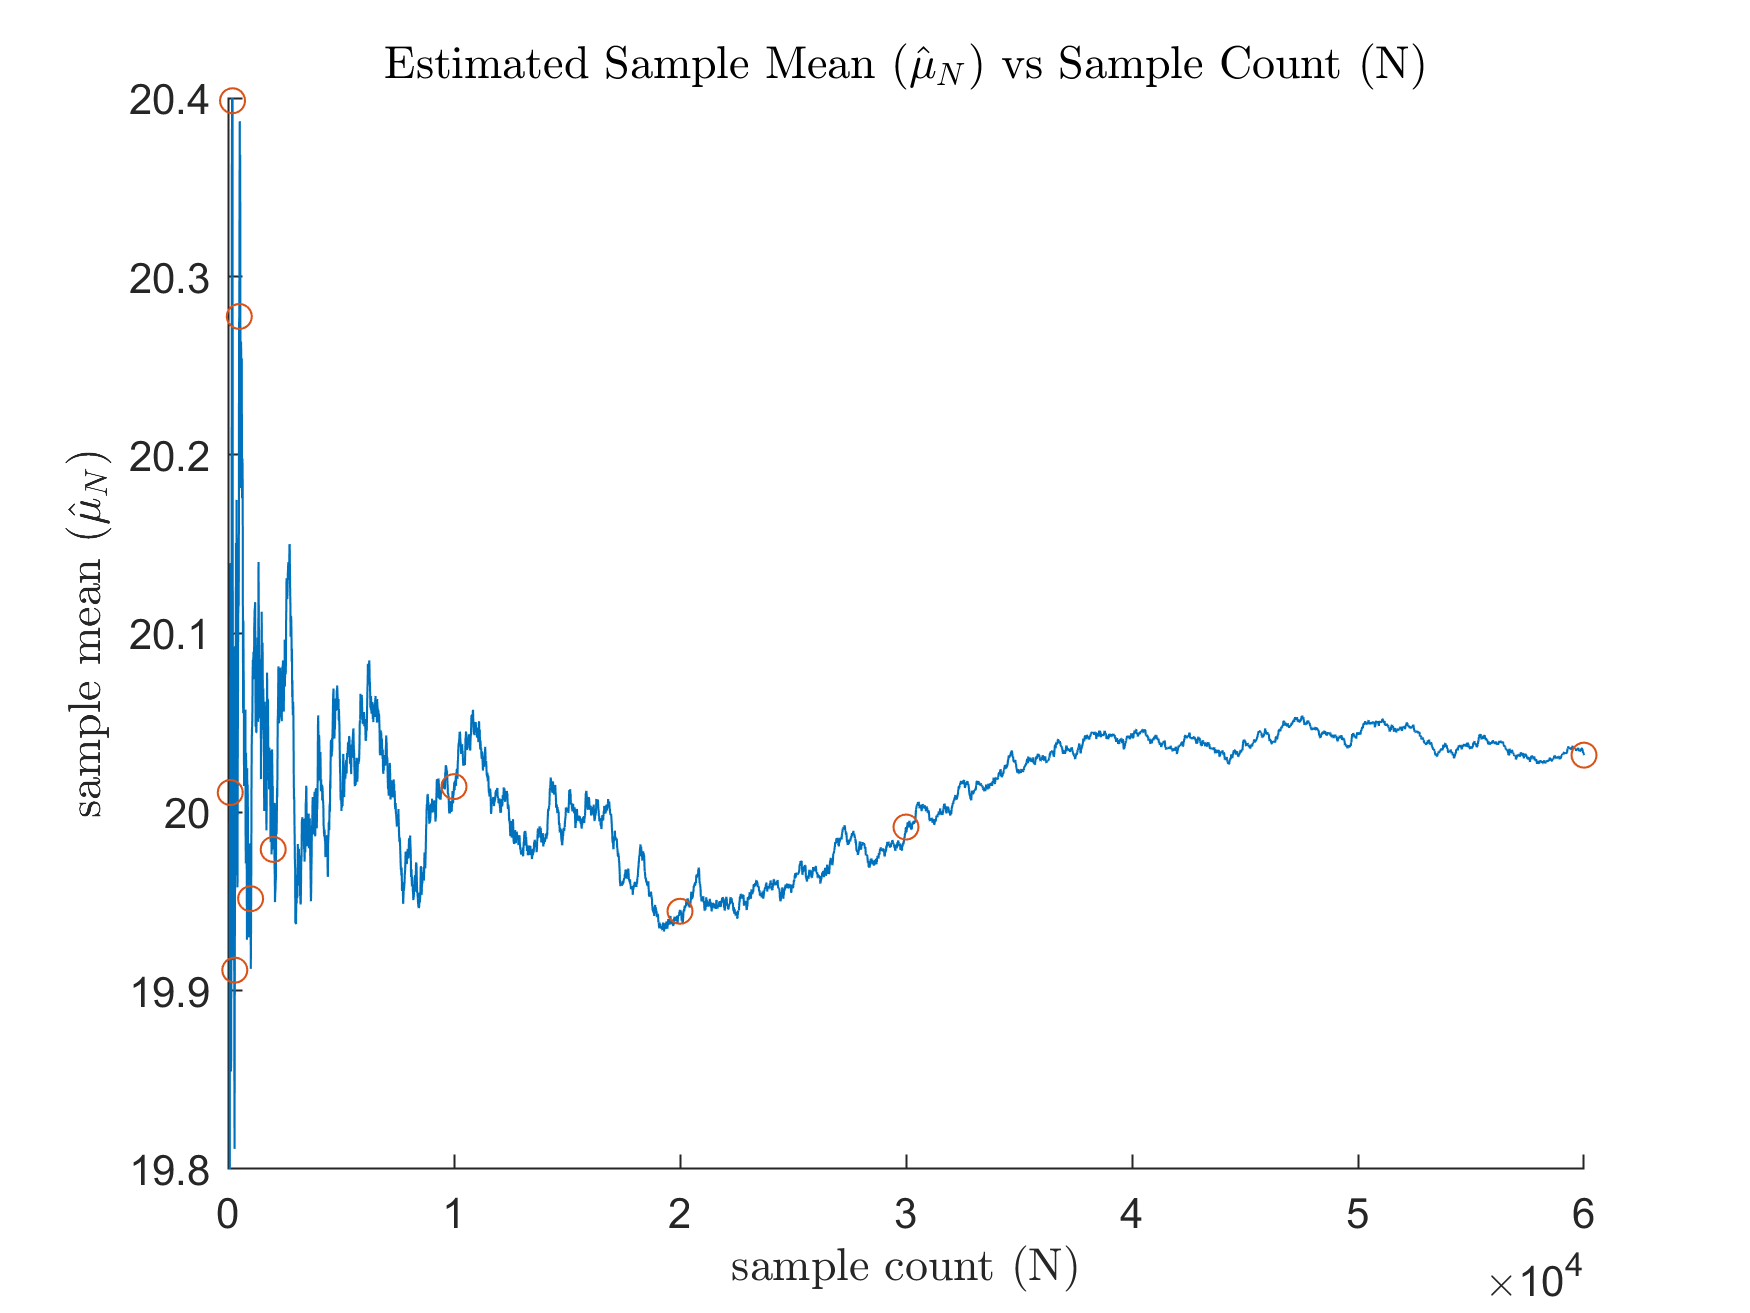
\includegraphics[scale=0.7, right]{01_b}
	\end{minipage}
	\caption{Sample means estimated from 10 to 60000 samples.}
	\label{fig:sample mean}
	\parskip 2pt
	$\hat{\mu}_N$ behaves erratically until the sample count reaches 100 samples, then fluctuates around a value of 20 $\pm$ 0.01. Hence, after 100 samples, $\hat{\mu}_N$ approaches the true mean.
\end{figure}

\pagebreak

\subsection{Sample mean accuracy $\hat{A}_N$ over $N$ samples}
\begin{figure}[h!]
	\begin{minipage}{0.25\textwidth}
		\begin{tabular}{| c | c |}
			\hline
			N & $\hat{A}_N$ \\
			\hline
			10 & 112.8127 \\
			20 & 105.1433 \\
			50 & 101.6648 \\
			100 & 99.1946 \\
			200 & 99.3591 \\
			300 & 99.2009 \\
			500 & 99.2756 \\
			1000 & 99.1960 \\
			2000 & 99.1945 \\
			10000 & 99.1948 \\
			20000 &	99.1966 \\
			30000 &	99.1943 \\
			60000 &	99.1958 \\
			\hline
		\end{tabular}
	\end{minipage}
	\begin{minipage}{0.7\textwidth}
		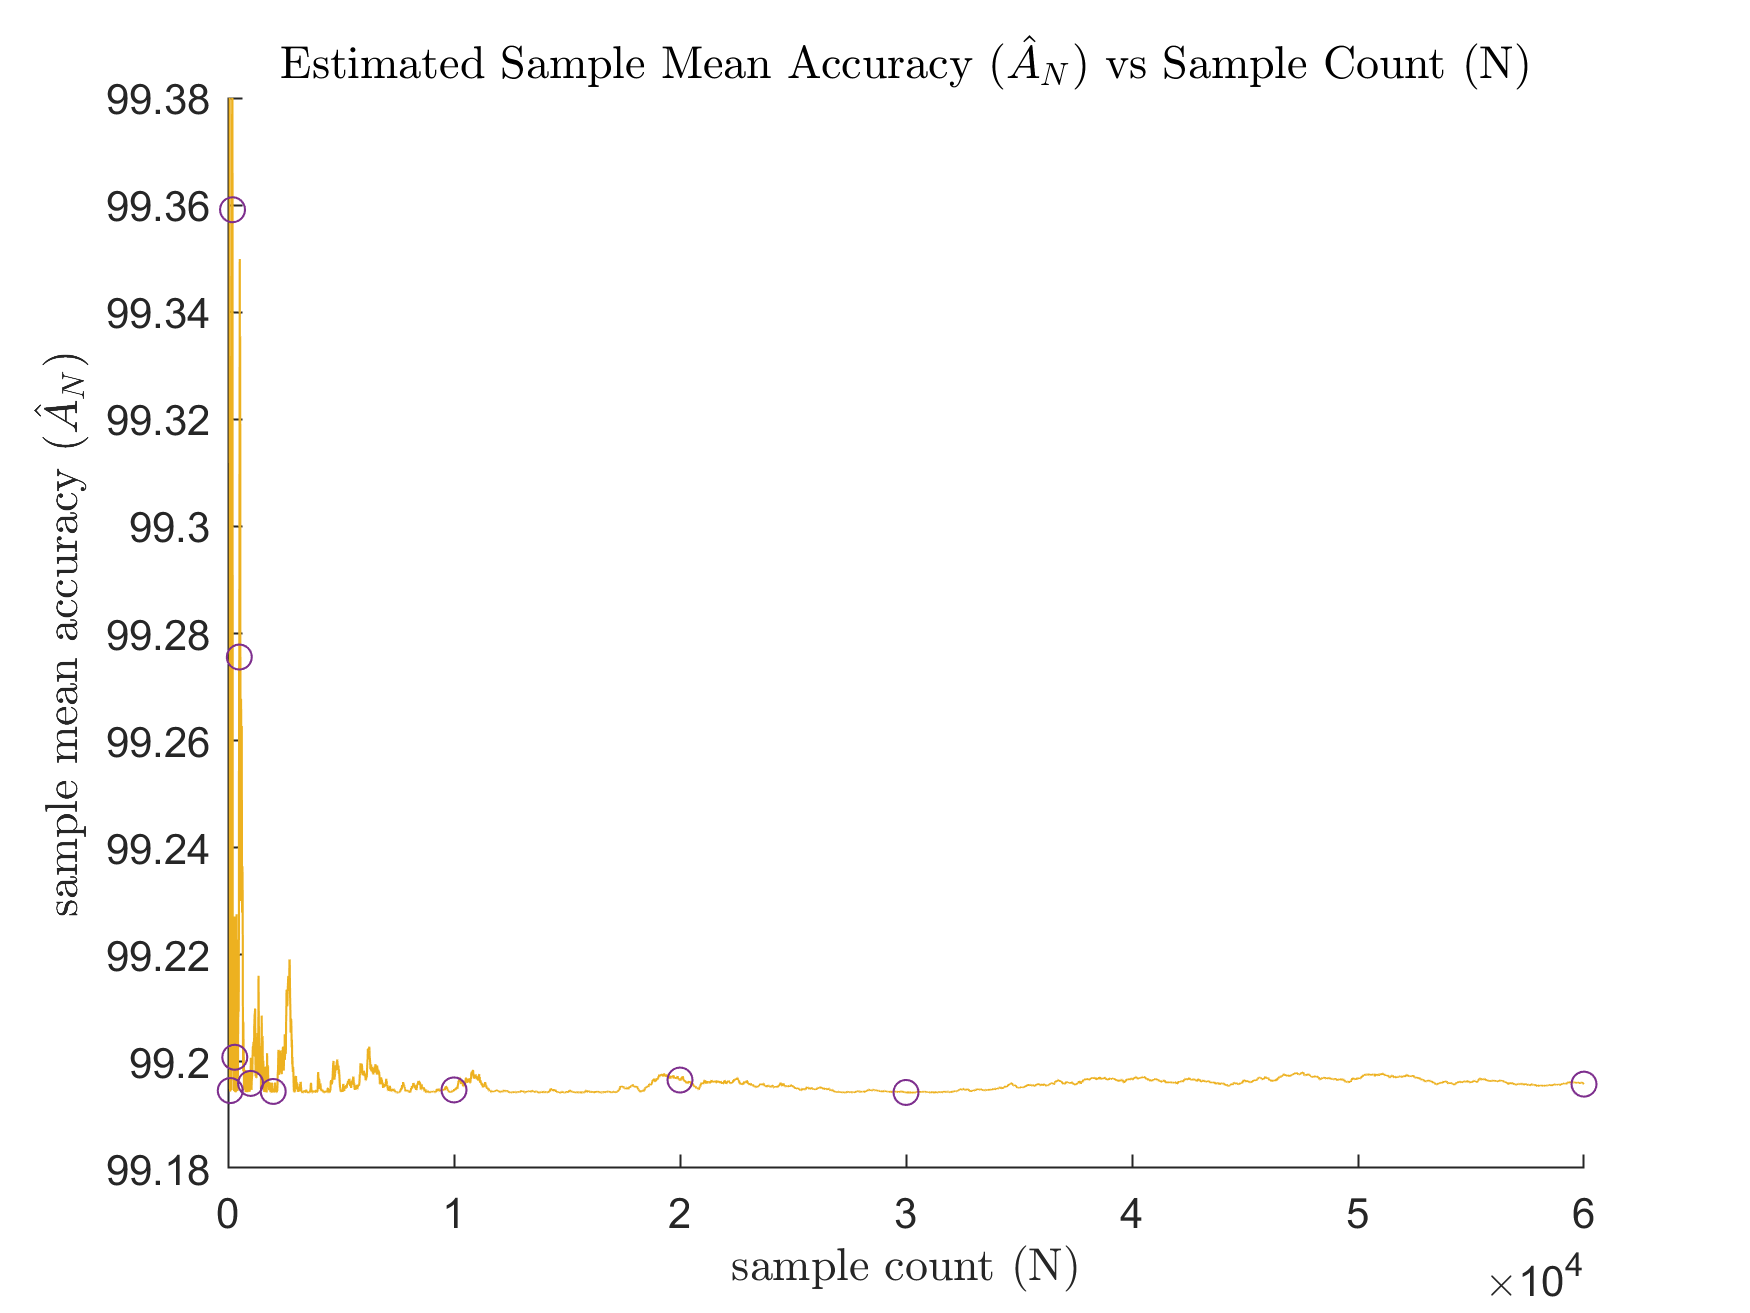
\includegraphics[scale=0.7, right]{01_c}
	\end{minipage}
	\caption{Sample mean accuracy estimated from 10 to 60000 samples.}
	\label{fig:sample mean accuracy}
	\parskip 2pt
	As the sample count reaches 1000 samples, $\hat{A}_N$ fluctuates approximately between 112 and 99.2. From 10000 to 60000 samples, $\hat{A}_N$ approaches 99.2. After 10000 samples and as $\hat{\mu}_N$ approaches the true mean, $\hat{A}_N$ reaches an approximate value.  
\end{figure}

\subsection{Limiting Value of $\hat{A}_N$}
As $N$ approaches a large number, based on figure \ref{fig:sample mean accuracy}, $\hat{A}_N$ approaches the value of 99.2. Since $\hat{\mu}_N$ approaches the true mean as $N$ approaches a large number and the random variable $X_i$ is positive, the difference between each sample and the true mean is non-negative. Additionally, since the data samples are not identical, the limiting value of $\hat{A}_N$ is not zero.

\subsection{Estimation of $\sigma^2$}
Based on the limiting value of $\hat{A}_N$, the variance is approximately 99.2.

\pagebreak

\section{Central Limit Theorem}

\subsection{PDF \& CDF of the mean $M_n$ of a sequence of i.i.d. RVs}

\begin{figure}[h!]
	\centering
	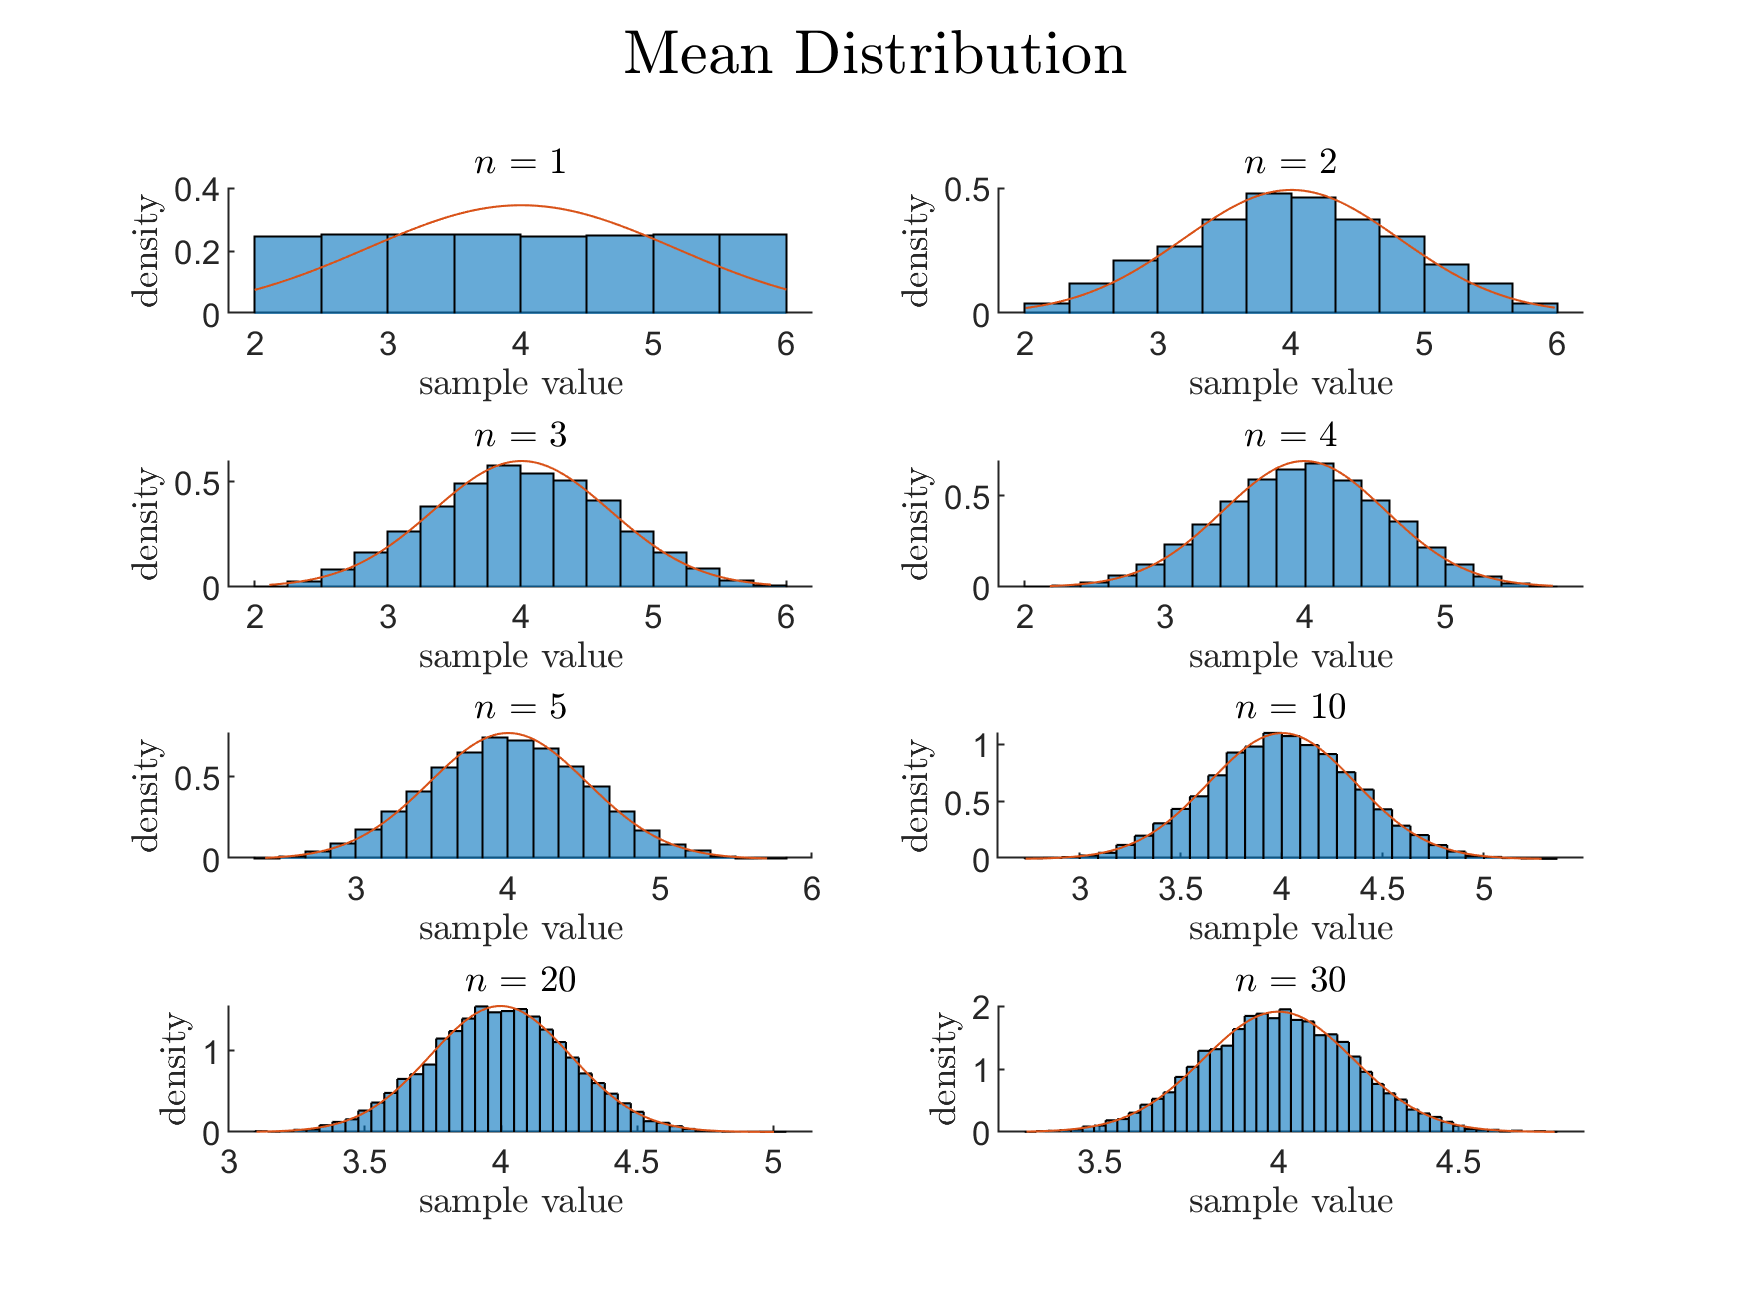
\includegraphics[scale=0.95]{02_a_pdf}
	\vspace{-24pt}
	\caption{PDF of $M_n$ for $n \in \{1,2,3,4,5,10,20,30\}$.} 
	\label{fig:mean pdf}
	\vspace{16pt}
	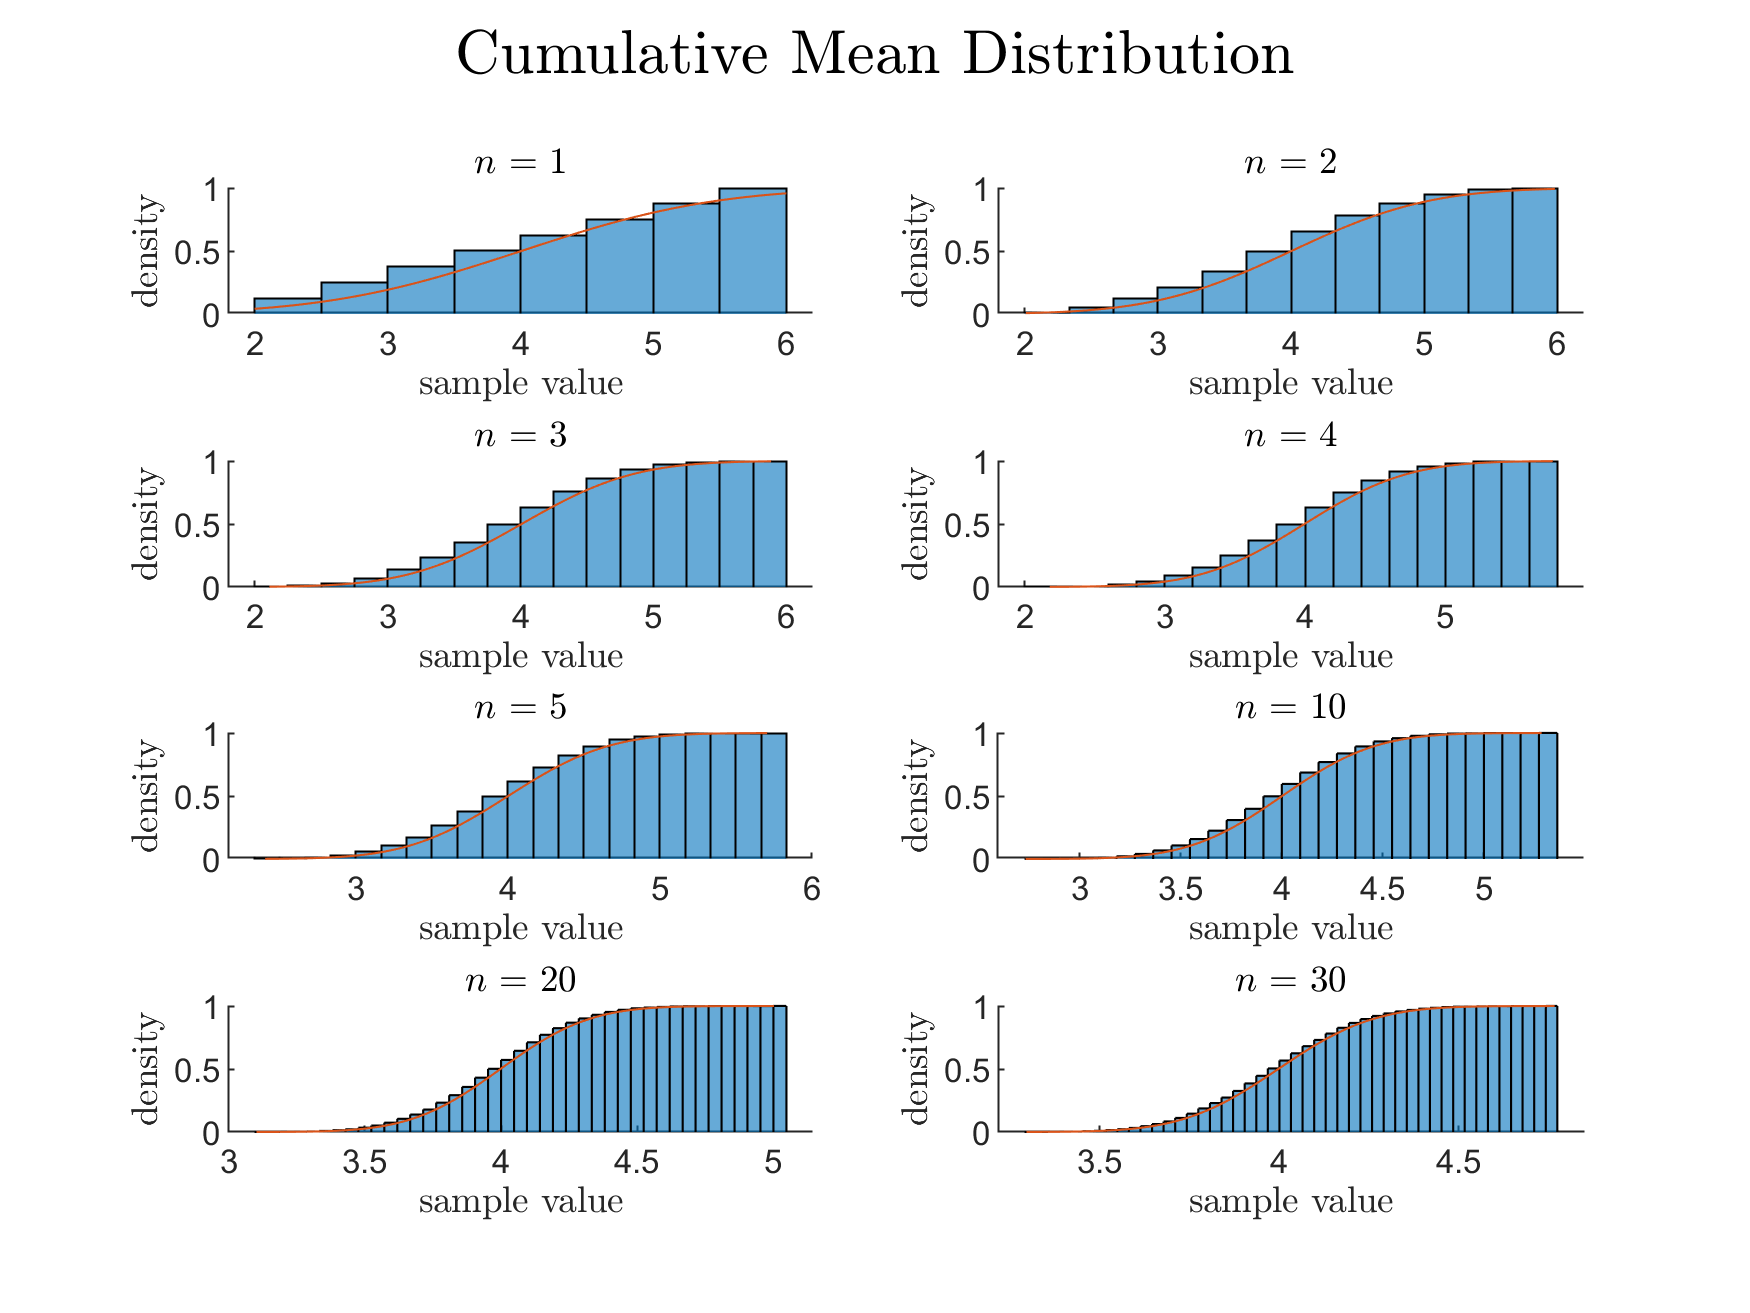
\includegraphics[scale=0.95]{02_a_cdf}
	\vspace{-24pt}
	\caption{CDF of $M_n$ for $n \in \{1,2,3,4,5,10,20,30\}$.}
	\label{fig:mean cdf}
\end{figure}

\pagebreak

\begin{flushleft}
Based on the histograms, the mean and cumulative mean distributions of $M_n$ approach the pdf and cdf of a Gaussian RV as $n$ increases. The results show that the pdf and cdf of the sum of a sequence of i.i.d. RVs follows the pdf and cdf distributions of a Gaussian RV.
\end{flushleft}

\subsection{Mean and Variance of $X_i$ and $M_n$}

\subsubsection{Mean and Variance of $X_i$}
According to the prompt given, the mean of $X_i$ is equal to $\mu$ and the variance of $X_i$ is equal to $\sigma^2 \; \forall \; i \in \{1,2,3,\dots,n\}$.

\subsubsection{Mean of $M_n$}
\begin{align}
	\text{E}[M_n] &= \text{E}[\frac{X_1+X_2+\dots+X_n}{n}] &\text{by the definition of the expectation}	
	\\
	&= \frac{\text{E}[X_1]+\text{E}[X_2]+\dots+\text{E}[X_n]}{\text{E}[n]}	&\text{by the linearity of expectation}
	\\
	&= \frac{\mu+\mu+\dots+\mu}{\text{E}[n]}	&\text{since E$[X_i]=\mu \; \forall \; i$}
	\\
	&= \frac{\mu+\mu+\dots+\mu}{n}	&\text{by the expected value of a constant}
	\\
	&= \frac{n\mu}{n}
	\\
	&= \mu
\end{align}
	
\subsubsection{Variance of $M_n$}
\begin{align}
	Var(M_n) &= Var(\frac{X_1+X_2+\dots+X_n}{n}) &\text{by the definition of $M_n$}
	\\
	&= \frac{1}{n^2}Var(X_1+X_2+\dots+X_n) &\text{since $Var(aX)=a^2Var(X)$}
	\\
	&= \frac{1}{n^2}[Var(X_1)+Var(X_2)+\dots+Var(X_n)] &\text{since $X_j \perp\!\!\!\perp X_k \; \forall \; j \neq k$}
	\\
	&= \frac{1}{n^2}[\sigma^2 + \sigma^2 + \dots + \sigma^2] &\text{since $Var[X_i]=\sigma^2 \; \forall \; i$}
	\\
	&= \frac{n\sigma^2}{n^2} 
	\\
	&= \frac{\sigma^2}{n}
\end{align}

\pagebreak

\subsection{Multivariate Gaussian RV}

\begin{figure}[h!]
	\centering
	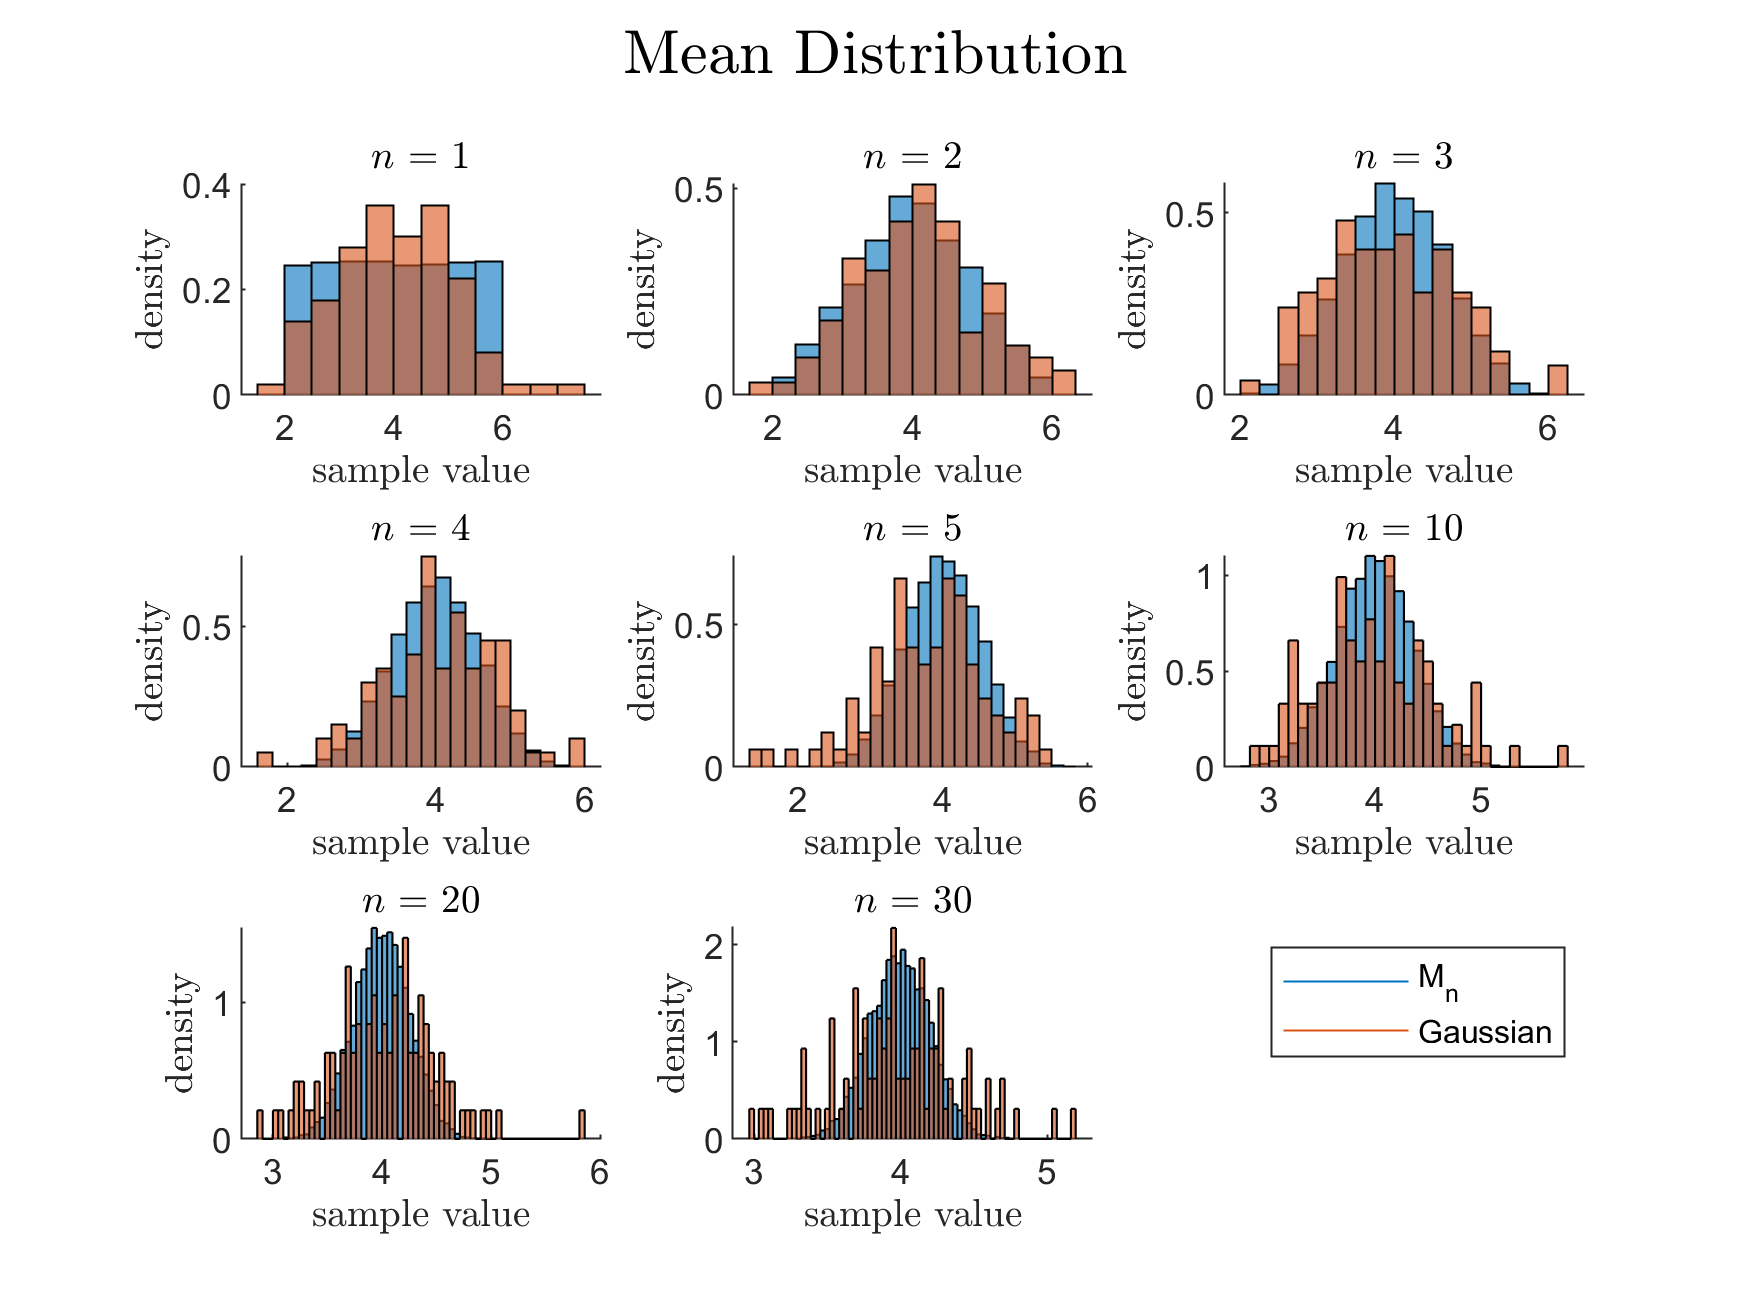
\includegraphics{02_c_pdf}
	\vspace{-24pt}
	\caption{PDF of $M_n$ and a Multivariate Gaussian for $n \in \{1,2,3,4,5,10,20,30\}$.} 
	\label{fig:gaussian pdf}
	\vspace{16pt}
	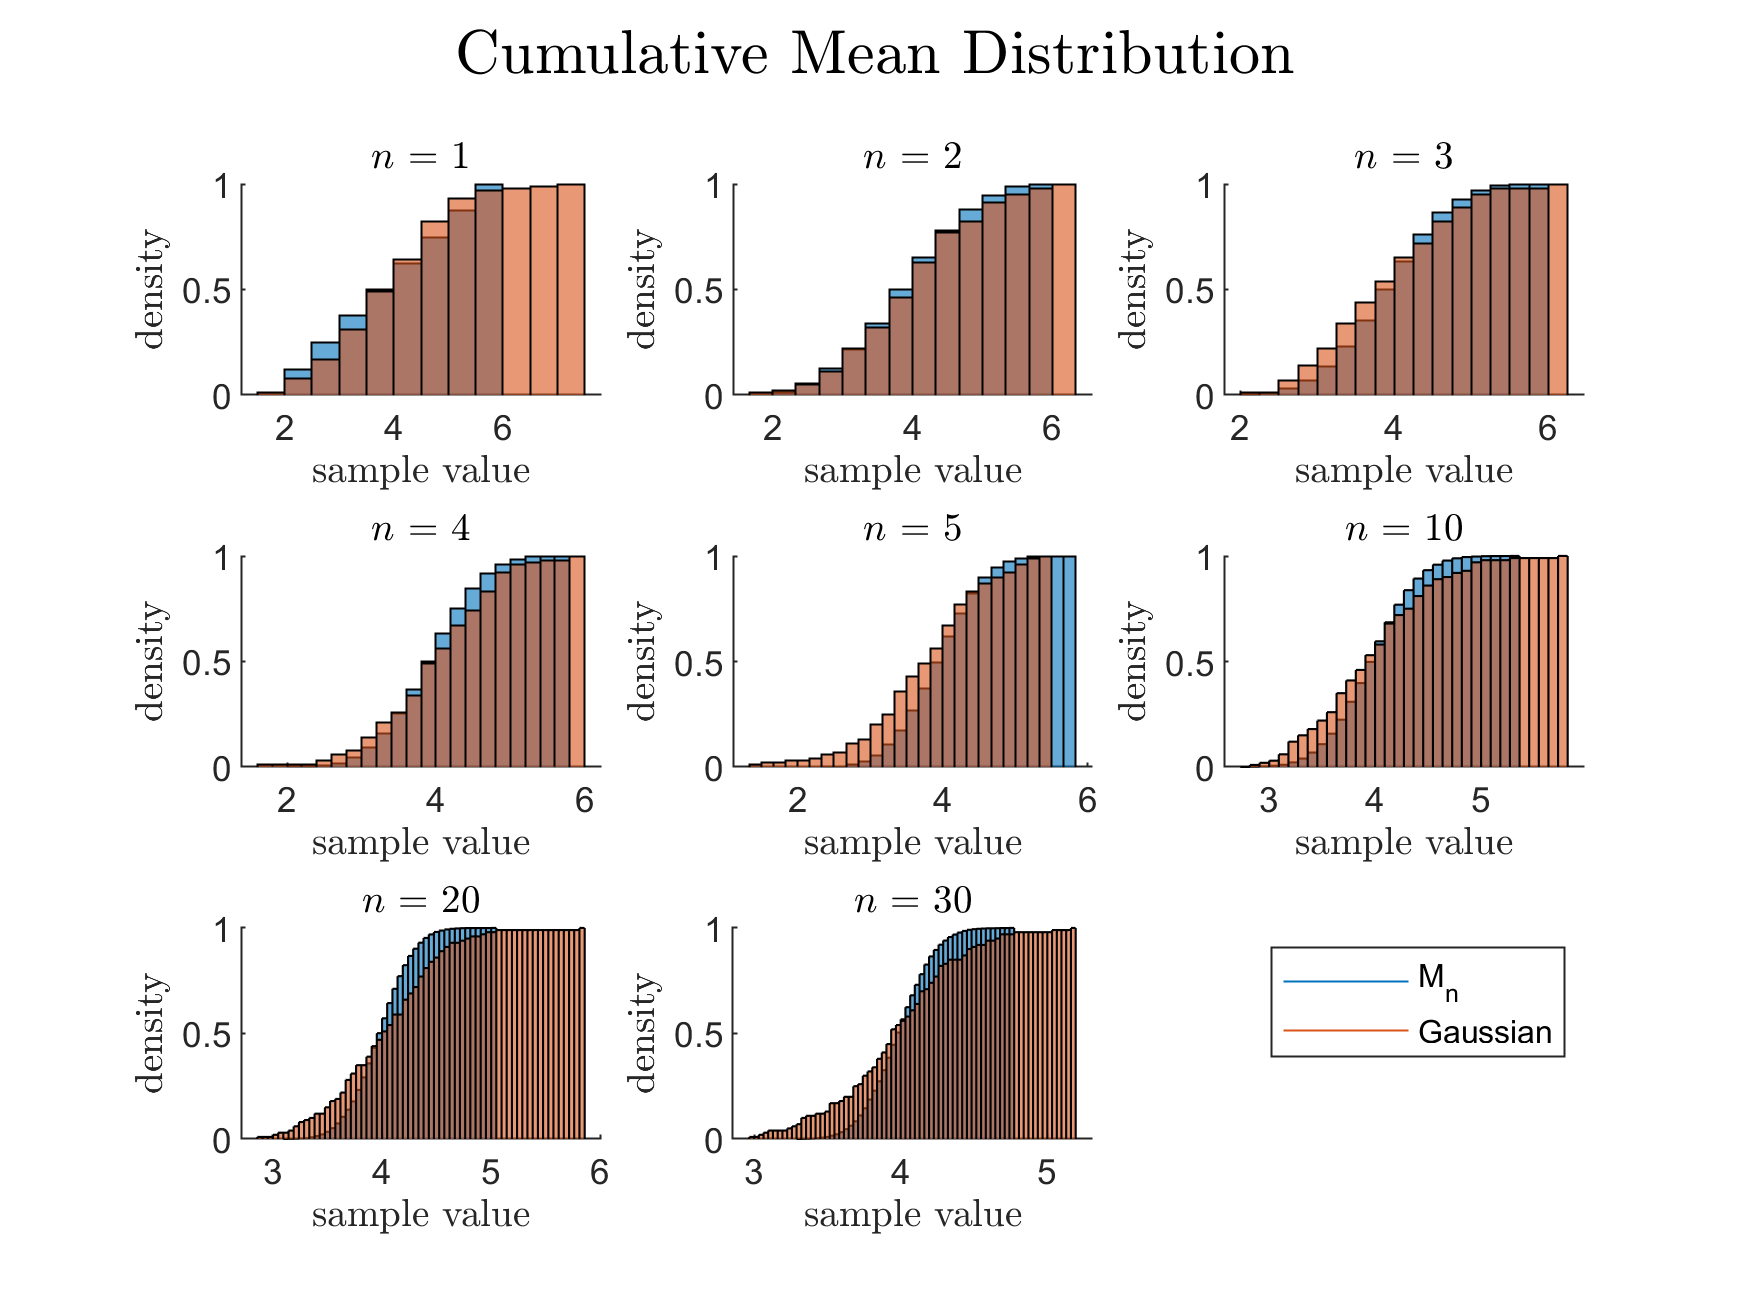
\includegraphics{02_c_cdf}
	\vspace{-24pt}
	\caption{CDF of $M_n$ and a Multivariate Gaussian for $n \in \{1,2,3,4,5,10,20,30\}$.}
	\label{fig:gaussian cdf}
\end{figure}

\pagebreak 

\subsection{$X_i$ representing an unfair 5-sided dice}

\subsubsection{PDF \& CDF of the mean $M_n$ of a sequence of biased RVs}

\begin{figure}[h!]
	\centering
	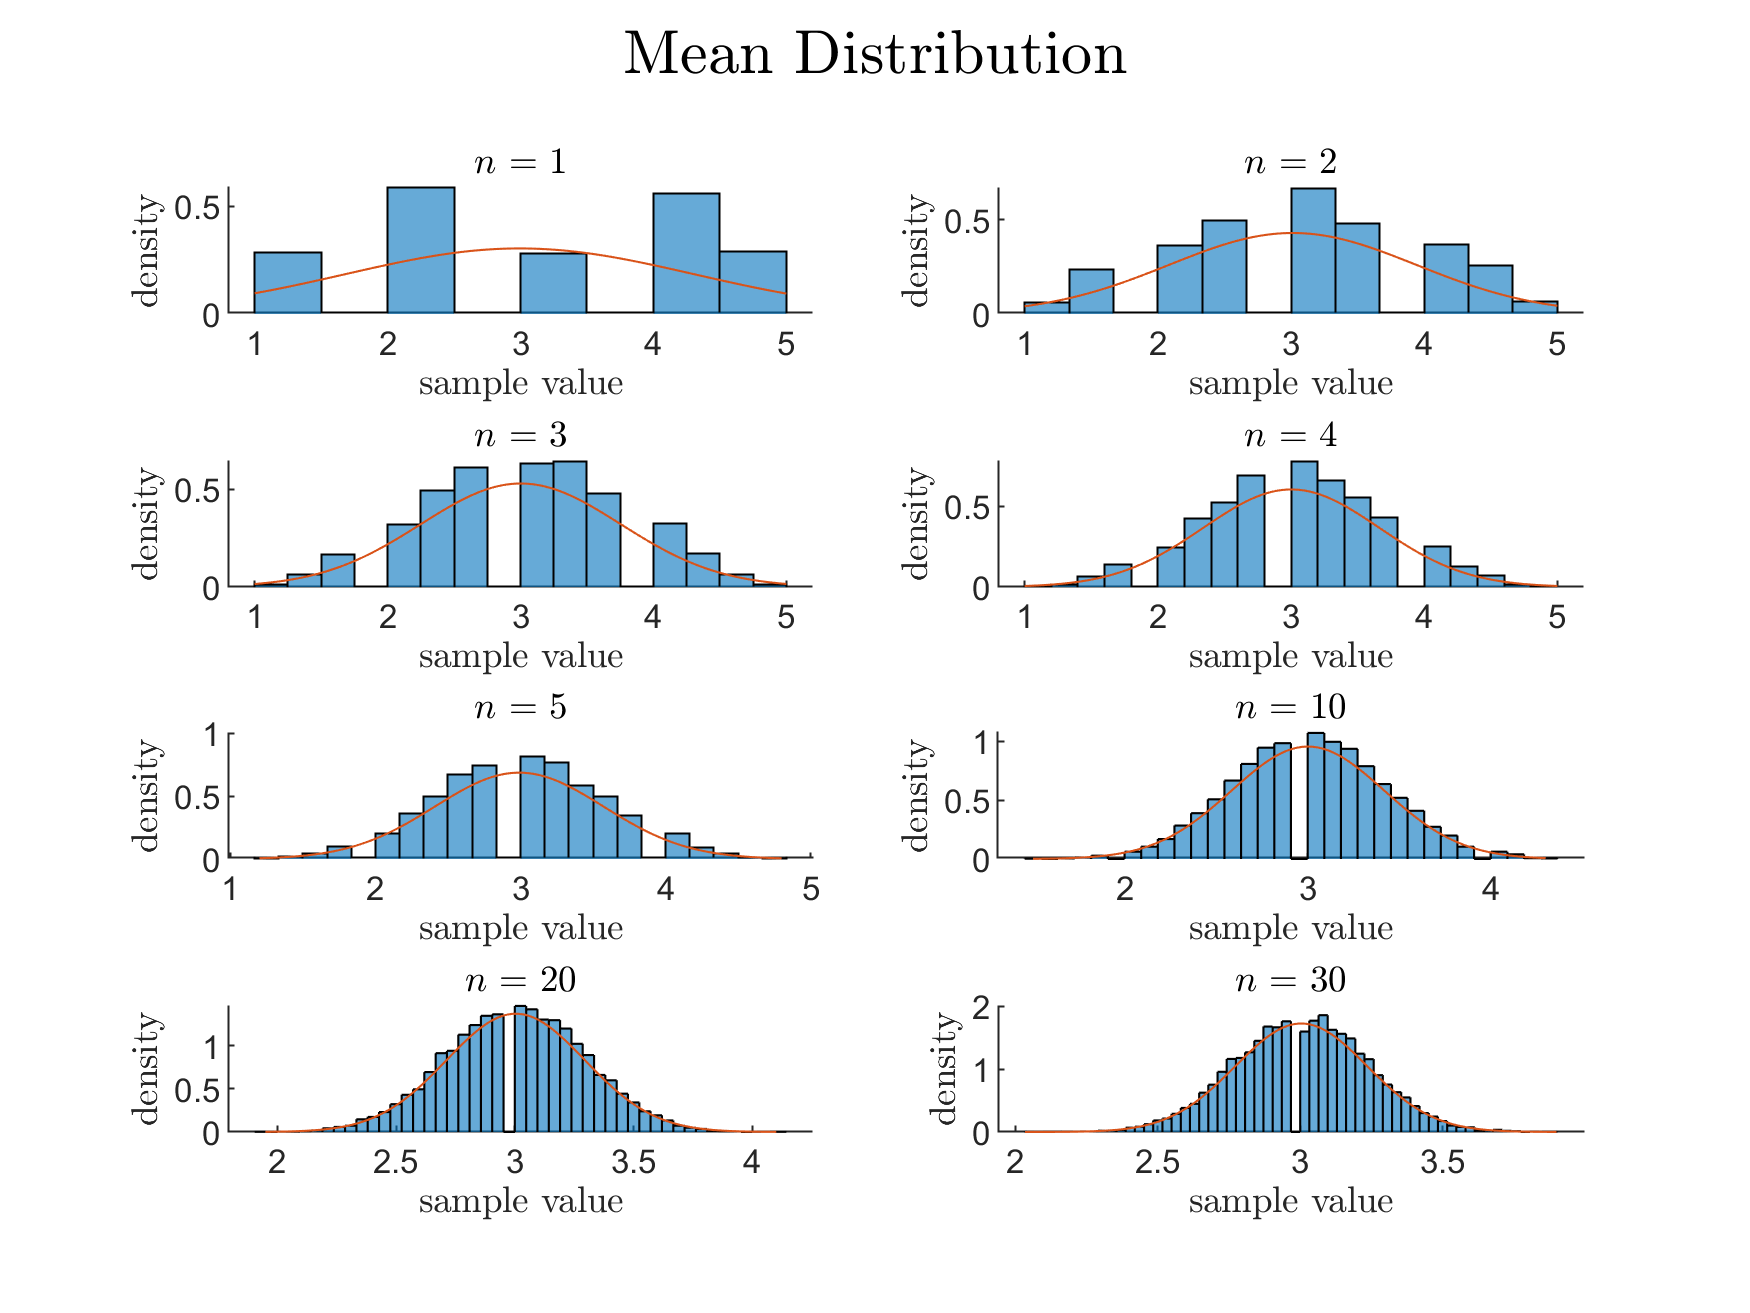
\includegraphics[scale=0.9]{02_d_a_pdf}
	\vspace{-24pt}
	\caption{PDF of $M_n$ for $n \in \{1,2,3,4,5,10,20,30\}$.} 
	\label{fig:biased mean pdf}
	\vspace{16pt}
	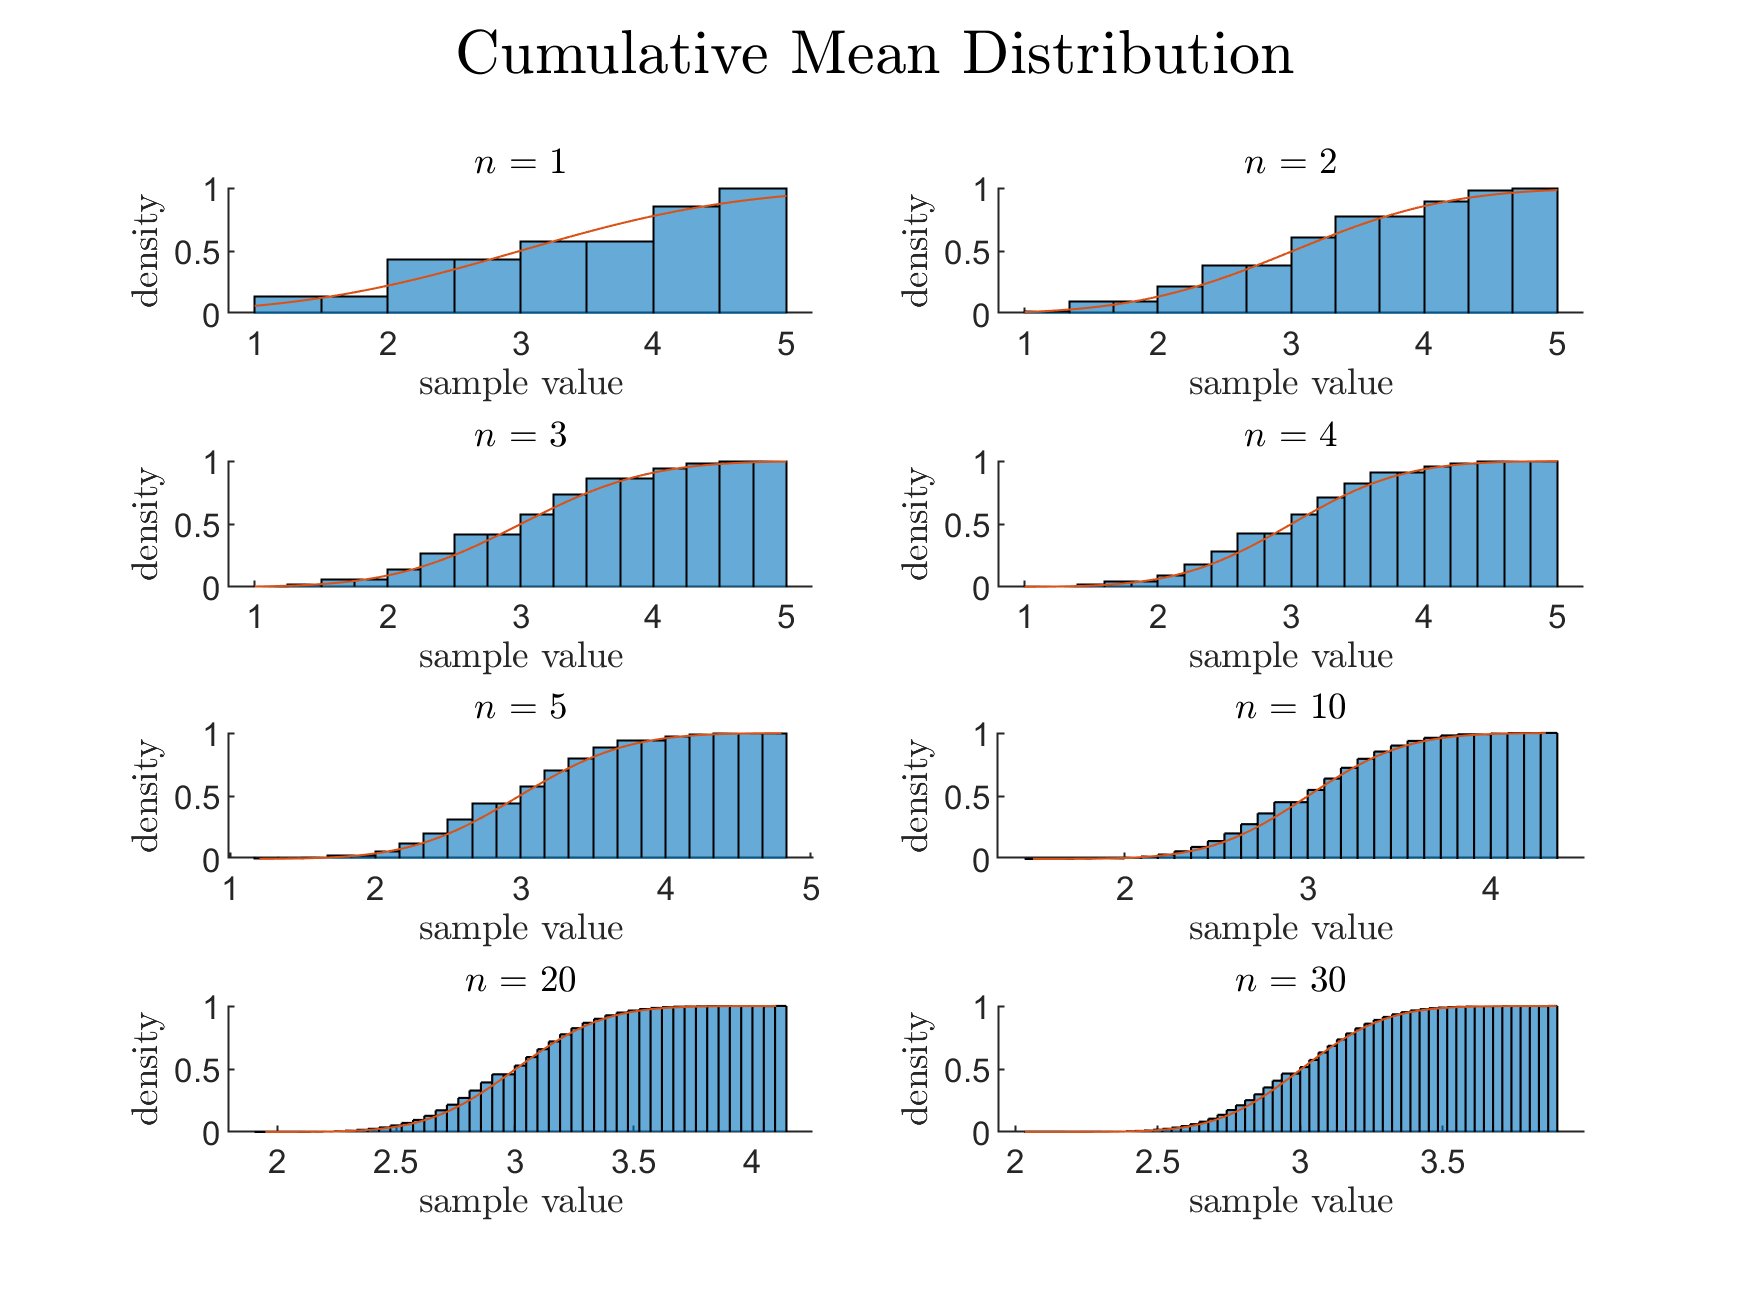
\includegraphics[scale=0.9]{02_d_a_cdf}
	\vspace{-24pt}
	\caption{CDF of $M_n$ for $n \in \{1,2,3,4,5,10,20,30\}$.}
	\label{fig:biased mean cdf}
\end{figure}

\vspace{-8pt}

\begin{flushleft}
The histograms show the same Gaussian distributions as the last section. However, the pdf and cdf indicate bias for even sample values as indicated by the bimodal peaks in the pdf and the rise of the distribution for even-valued bins. 
\end{flushleft}

\subsubsection{Mean and Variance of $X_i$ and $M_n$}

\paragraph{2.4.2.1\quad Mean of $X_i$}
\begin{align}
	\text{E}[X_i] &= \sum_{i=1}^{5} x_i P(x=x_i) &\text{by the definition of expectation}
	\\
	&= 1 \cdot p + 2 \cdot 2p + 3 \cdot p + 4 \cdot 2p + 5 \cdot p &\text{by the pmf of an unfair 5-sided dice}
	\\
	&= 21 \cdot p
	\\
	&= 21 \cdot \frac{1}{7}	&\text{since $p=\frac{1}{7}$ for $\sum_{i=1}^{5} \text{P}(x=x_i) = 1$}
	\\
	&= 3
\end{align}

\paragraph{2.4.2.2\quad Variance of $X_i$}
\begin{align}
	\text{E}[X_i^2] &= \sum_{i=1}^{5} x_i^2 P(x=x_i)
	\\
	&= 1^2 \cdot p + 2^2 \cdot 2p + 3^2 \cdot p + 4^2 \cdot 2p + 5^2 \cdot p
	\\
	&= 75 \cdot p
	\\
	&= \frac{75}{7}	
\end{align}

\vspace{-16pt}

\begin{align}
	Var(X_i) &= \text{E}[X_i^2]-(\text{E}[X_i])^2 \hspace{3.2cm} &\text{by the definition of variance}
	\\
	&= \frac{75}{7} - 3^2
	\\
	&= \frac{12}{7}
\end{align}

\paragraph{2.4.2.3\quad Mean of $M_n$}
\begin{align}
	\text{E}[M_n] &= \text{E}[\frac{X_1+X_2+\dots+X_n}{n}] &\text{by the definition of the expectation}	
	\\
	&= \frac{\text{E}[X_1]+\text{E}[X_2]+\dots+\text{E}[X_n]}{\text{E}[n]}	&\text{by the linearity of expectation}
	\\
	&= \frac{3+3+\dots+3}{\text{E}[n]}	&\text{since E$[X_i]=3 \; \forall \; i \in \{1,2,3,\dots,n\}$}
	\\
	&= \frac{3+3+\dots+3}{n}	&\text{by the expected value of a constant}
	\\
	&= \frac{n \cdot 3}{n}
	\\
	&= 3
\end{align}
	
\paragraph{2.4.2.4\quad Variance of $M_n$}
\begin{align}
	Var(M_n) &= Var(\frac{X_1+X_2+\dots+X_n}{n}) &\text{by the definition of $M_n$}
	\\
	&= \frac{1}{n^2}Var(X_1+X_2+\dots+X_n) &\text{since $Var(aX)=a^2Var(X)$}
	\\
	&= \frac{1}{n^2}[Var(X_1)+Var(X_2)+\dots+Var(X_n)] &\text{since $X_j \perp\!\!\!\perp X_k$ for $j \neq k$}
	\\
	&= \frac{1}{n^2}[\frac{12}{7} + \frac{12}{7} + \dots + \frac{12}{7}] &\text{since $Var[X_i]=\frac{12}{7} \; \forall \; i$}
	\\
	&= \frac{12n}{7n^2} 
	\\
	&= \frac{12}{7n}
\end{align}

\subsubsection{Multivariate Gaussian RV}

\begin{figure}[h!]
	\centering
	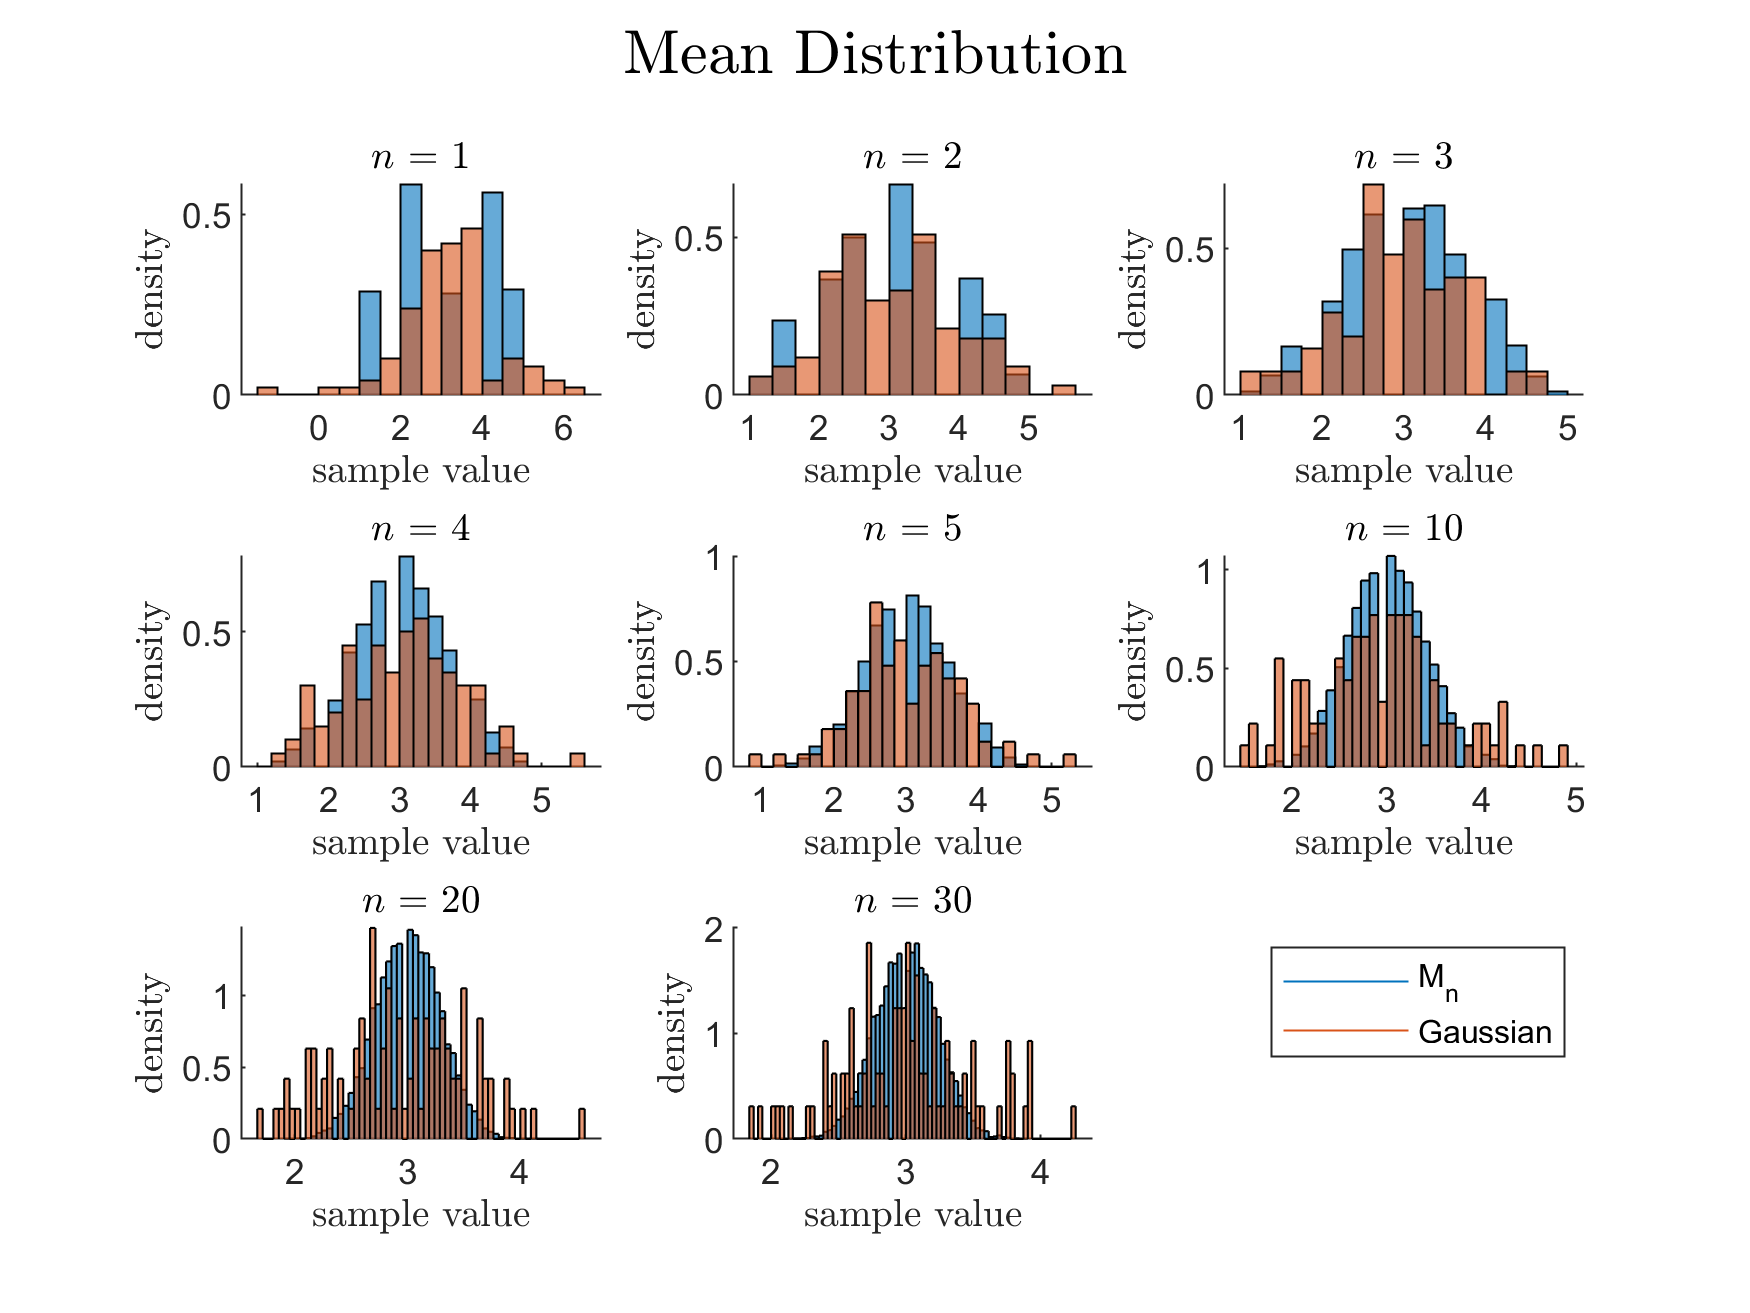
\includegraphics{02_d_c_pdf}
	\caption{PDF of $M_n$ and a Multivariate Gaussian for $n \in \{1,2,3,4,5,10,20,30\}$.} 
	\label{fig:biased gaussian pdf}
\end{figure}

\pagebreak

\begin{figure}[h!]
	\centering
	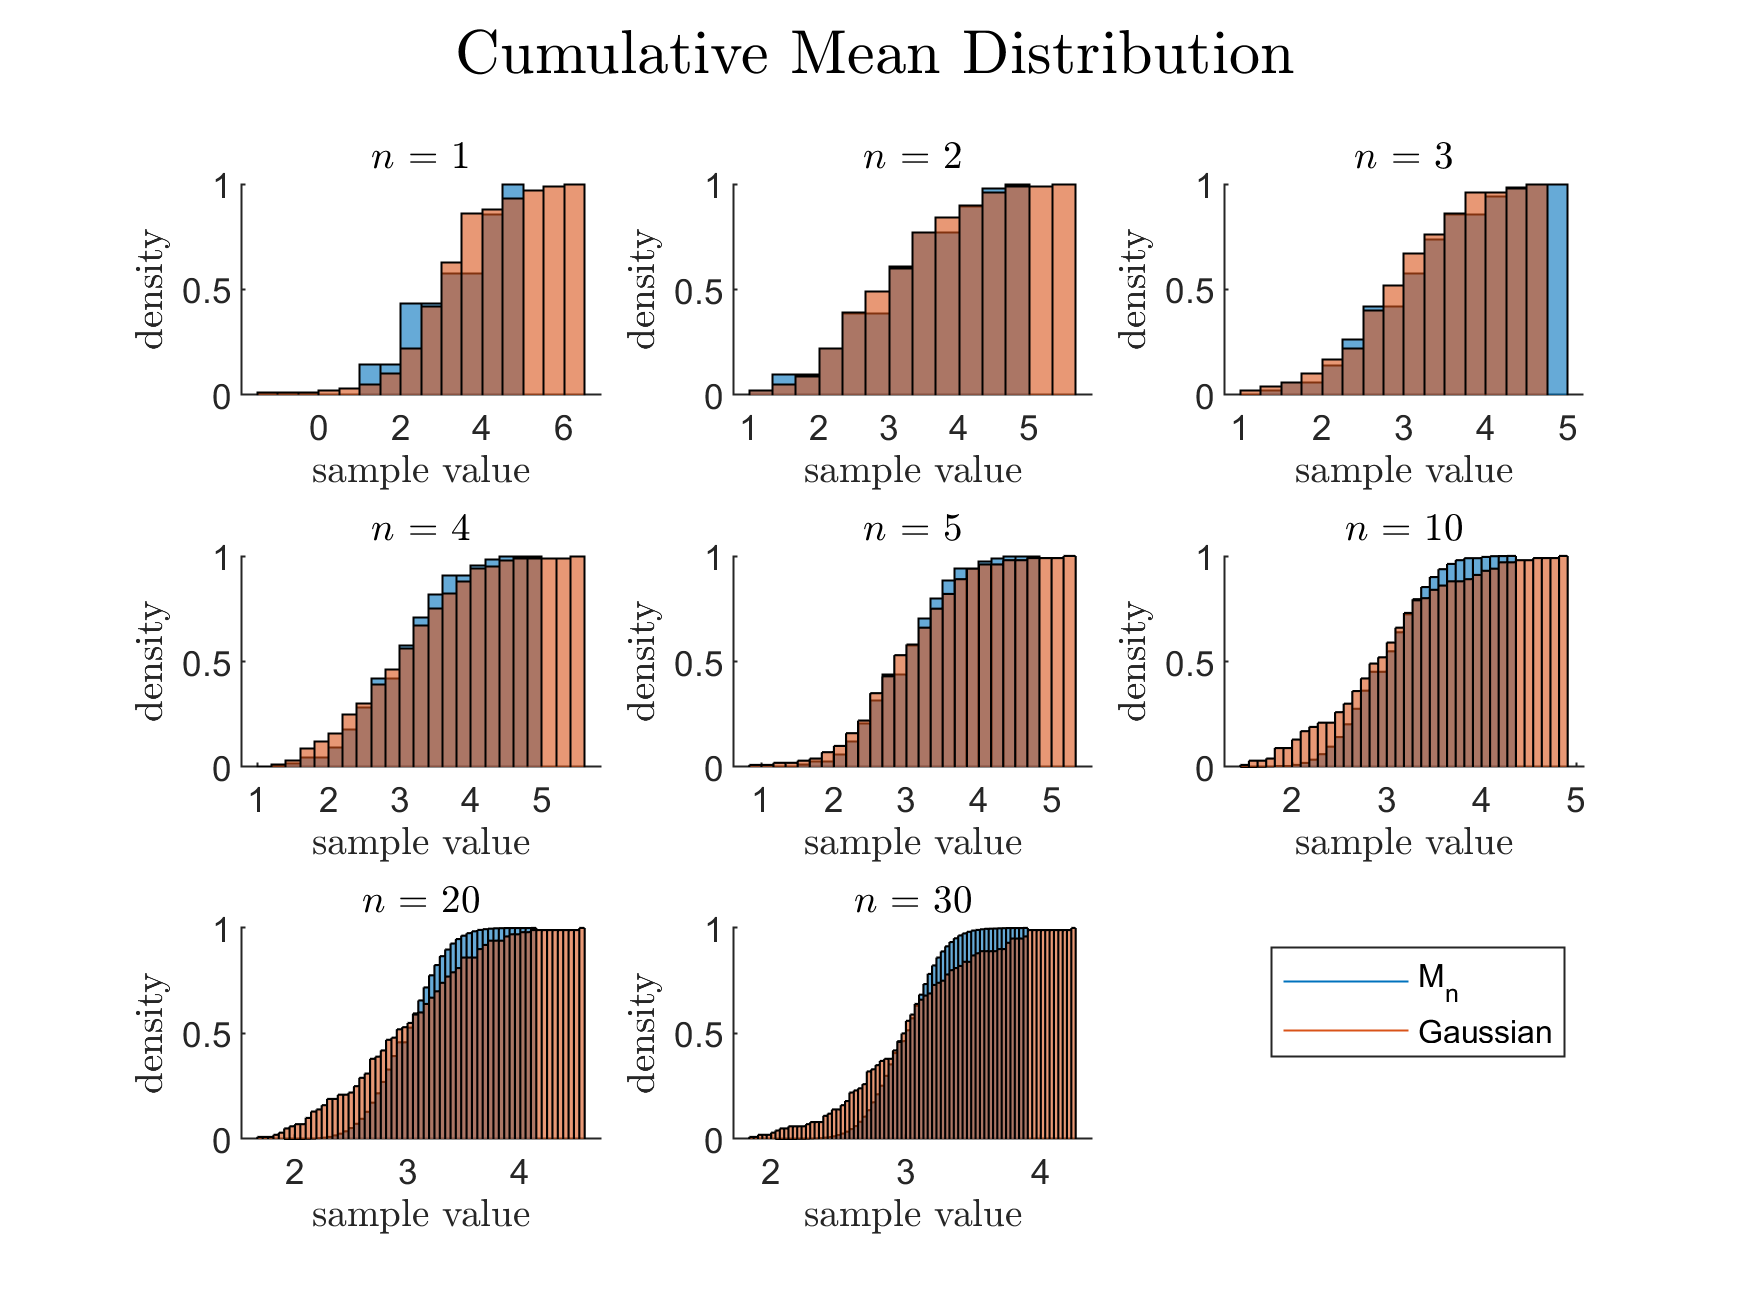
\includegraphics{02_d_c_cdf}
	\caption{CDF of $M_n$ and a Multivariate Gaussian for $n \in \{1,2,3,4,5,10,20,30\}$.}
	\label{fig:biased gaussian cdf}
\end{figure}

\pagebreak 

\section{Gaussian Discriminant Analysis}

\subsection{Classification Rule for $\sum = \sum_0 = \sum_1$ and $p=\frac{1}{2}$}

\begin{align}
	P(y=0|\vec{x}) & \geq P(y=1|\vec{x})
	\\
	\frac{P(\vec{x}|y=0)P(y=0)}{P(\vec{x})} & \geq \frac{P(\vec{x}|y=1)P(y=1)}{P(\vec{x})} & \text{by Bayes' Rule}
	\\
	P(\vec{x}|y=0)P(y=0) & \geq P(\vec{x}|y=1)P(y=1)
	\\
	\frac{1}{2}P(\vec{x}|y=0) & \geq \frac{1}{2}P(\vec{x}|y=1) & \text{since }
	y=
		\begin{cases}
			1	& \text{w.p. } p
			\\
			0	& \text{w.p. } 1-p
		\end{cases}
	\\
	P(\vec{x}|y=0) & \geq P(\vec{x}|y=1)
	\\
	f_{X,y=0}(\vec{x}) & \geq f_{X,y=1}(\vec{x})
\end{align}

\begin{align}
	f_{X}(\vec{x}) &= \frac{\text{exp}\{-\frac{1}{2}(\vec{x}-\mu)^T K^{-1}(\vec{x}-\mu)\}}{(2\pi)^{\frac{n}{2}}|K|^\frac{1}{2}}
	& \text{by the definition of a Gaussian pdf} 
\end{align}

\begin{align}
	K &= 
	\begin{bmatrix}
		Var(X_1)     & Cov(X_1,X_2) & \dots & Cov(X_1,X_n) \\
		Cov(X_2,X_1) & Var(X_2)     & \dots & Cov(X_2,X_n) \\
		\vdots		 & \vdots		& 		& \vdots	   \\
		Cov(X_n,X_1) & \dots		& 		& Var(X_n)
	\end{bmatrix}
	\\
	&= 
	\begin{bmatrix}
		Var(X_1)     & 0			& \dots & 0			   \\
		0			 & Var(X_2)     & \dots & 0			   \\
		\vdots		 & \vdots		& 		& \vdots	   \\
		0			 & \dots		& 		& Var(X_n)
	\end{bmatrix}
	\hspace{12pt}
	\text{since $\rho = 0$ for $X_j \perp\!\!\!\perp X_k$ for $j \neq k$}
	\\
	&= 
	\begin{bmatrix}
		\sum	     & 0			& \dots & 0			   \\
		0			 & \sum		    & \dots & 0			   \\
		\vdots		 & \vdots		& 		& \vdots	   \\
		0			 & \dots		& 		& \sum
	\end{bmatrix}
\end{align}

\begin{align}
	K^{-1} &= \frac{1}{\sum}
	\begin{bmatrix}
		1		     & 0			& \dots & 0			   \\
		0			 & 1		    & \dots & 0			   \\
		\vdots		 & \vdots		& 		& \vdots	   \\
		0			 & \dots		& 		& 1
	\end{bmatrix}
	\\
	&= \frac{I}{\sum}
\end{align}

\pagebreak

\begin{align}
	f_{X}(\vec{x}) &= \frac{\text{exp}\{-\frac{1}{2}(\vec{x}-\mu)^T \frac{I}{\sum} (\vec{x}-\mu)\}}{(2\pi)^{\frac{n}{2}}|\sum I|^\frac{1}{2}}
	\\
	&= \frac{\text{exp}\{-\frac{1}{2}(\vec{x}^T\Sigma^{-1}\vec{x}-\mu^T\Sigma^{-1}\vec{x}-x^T\Sigma^{-1}\mu+\mu^T\Sigma^{-1}\mu)\}}{(2\pi)^{\frac{n}{2}}|\sum|^\frac{1}{2}}
	& \text{cross multiply}
\end{align}

\begin{align}
	ln(\text{exp}) &= ln(\text{exp}\{-\frac{1}{2}(\vec{x}^T\Sigma^{-1}\vec{x}-\mu^T\Sigma^{-1}\vec{x}-x^T\Sigma^{-1}\mu+\mu^T\Sigma^{-1}\mu)\})
	\\
	&= -\frac{1}{2}(\vec{x}^T\Sigma^{-1}\vec{x}-\mu^T\Sigma^{-1}\vec{x}-x^T\Sigma^{-1}\mu+\mu^T\Sigma^{-1}\mu)
	\\
	&= -\frac{1}{2}(\vec{x}^T\Sigma^{-1}\vec{x}-2\mu^T\Sigma^{-1}\vec{x}+\mu^T\Sigma^{-1}\mu) & \hspace{-48pt} \text{since $\mu^T\Sigma^{-1}\vec{x}=x^T\Sigma^{-1}\mu$}
\end{align}

\begin{align}
	f_{X,y=0}(\vec{x}) &\geq f_{X,y=1}(\vec{x})
	\\
	-\frac{1}{2}(\vec{x}^T\Sigma^{-1}\vec{x}-2\mu_0^T\Sigma^{-1}\vec{x}+\mu_0^T\Sigma^{-1}\mu_0)
	& \geq
	-\frac{1}{2}(\vec{x}^T\Sigma^{-1}\vec{x}-2\mu_1^T\Sigma^{-1}\vec{x}+\mu_1^T\Sigma^{-1}\mu_1)
	\\
	\vec{x}^T\Sigma^{-1}\vec{x}-2\mu_0^T\Sigma^{-1}\vec{x}+\mu_0^T\Sigma^{-1}\mu_0
	& \geq
	\vec{x}^T\Sigma^{-1}\vec{x}-2\mu_1^T\Sigma^{-1}\vec{x}+\mu_1^T\Sigma^{-1}\mu_1
	\\
	-2\mu_0^T\Sigma^{-1}\vec{x}+2\mu_1^T\Sigma^{-1}\vec{x} 
	& \geq
	\mu_1^T\Sigma^{-1}\mu_1-\mu_0^T\Sigma^{-1}\mu_0
	\\
	[2(\mu_1-\mu_0)^T\Sigma^{-1}]\vec{x}+[\mu_0^T\Sigma^{-1}\mu_0-\mu_1^T\Sigma^{-1}\mu_1] &\geq 0
\end{align}

\subsection{Linear Inequality Contour for $\sum = \sum_0 = \sum_1$ and  $p=\frac{1}{2}$}

\begin{figure}[h!]
	\centering
	\vspace{-16pt}
	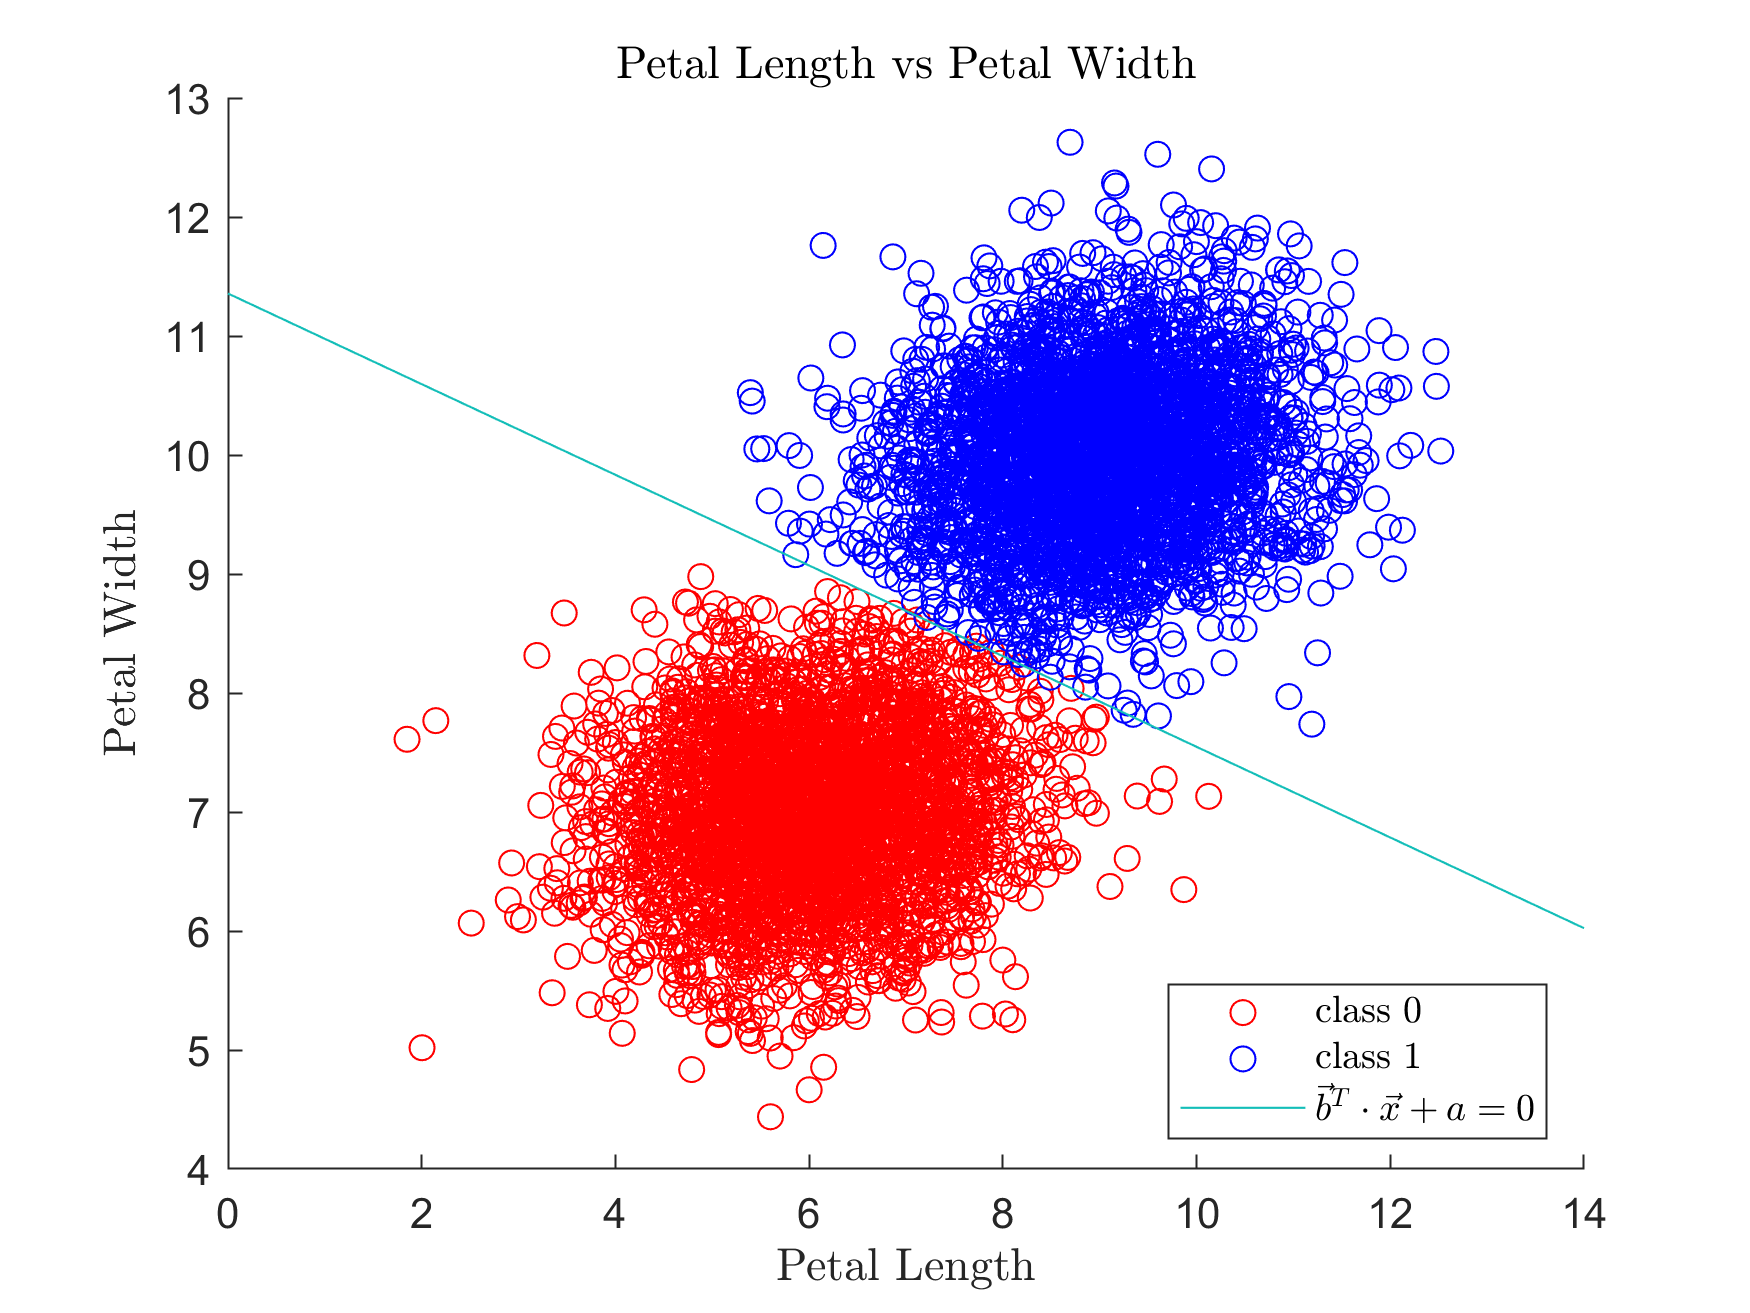
\includegraphics[scale=0.84]{03_b_scatter}
	\caption{Scatter plot and contour line of two classes from a sample with the same covariance and based on the linear inequality with $p=\frac{1}{2}$. Based on the samples, 50.17\% are categorized as class 0.} 
	\label{fig:contour for p=0.5}
\end{figure}

\subsection{Classification Rule for $\sum = \sum_0 = \sum_1$ and a general $p$}

\begin{align}
	P(y=0|\vec{x}) & \geq P(y=1|\vec{x})
	\\
	\frac{P(\vec{x}|y=0)P(y=0)}{P(\vec{x})} & \geq \frac{P(\vec{x}|y=1)P(y=1)}{P(\vec{x})} & \text{by Bayes' Rule}
	\\
	P(\vec{x}|y=0)P(y=0) & \geq P(\vec{x}|y=1)P(y=1)
	\\
	(1-p)P(\vec{x}|y=0) & \geq (p)P(\vec{x}|y=1) & \text{since }
	y=
		\begin{cases}
			1	& \text{w.p. } p
			\\
			0	& \text{w.p. } 1-p
		\end{cases}
	\\
	(1-p)f_{X,y=0}(\vec{x}) & \geq (p)f_{X,y=1}(\vec{x})
\end{align}

\begin{align}
	(1-p)f_{X,y=0}(\vec{x}) &\geq (p)f_{X,y=1}(\vec{x})
	\\
	\frac{\frac{1-p}{p}\text{exp}(\vec{x}^T\Sigma^{-1}\vec{x}-2\mu_0^T\Sigma^{-1}\vec{x}+\mu_0^T\Sigma^{-1}\mu_0)}{(2\pi)^{\frac{n}{2}}|\sum|^\frac{1}{2}}
	& \geq
	\frac{\text{exp}(\vec{x}^T\Sigma^{-1}\vec{x}-2\mu_1^T\Sigma^{-1}\vec{x}+\mu_1^T\Sigma^{-1}\mu_1)}{(2\pi)^{\frac{n}{2}}|\sum|^\frac{1}{2}}
\end{align}

\begin{align}
	\frac{(1-p)}{p}\text{exp}(\vec{x}^T\Sigma^{-1}\vec{x}-2\mu_0^T\Sigma^{-1}\vec{x}+\mu_0^T\Sigma^{-1}\mu_0-\vec{x}^T\Sigma^{-1}\vec{x}+2\mu_1^T\Sigma^{-1}\vec{x}-\mu_1^T\Sigma^{-1}\mu_1)
	& \geq 1
	\\
	\frac{(1-p)}{p}\text{exp}(-2\mu_0^T\Sigma^{-1}\vec{x}+\mu_0^T\Sigma^{-1}\mu_0+2\mu_1^T\Sigma^{-1}\vec{x}-\mu_1^T\Sigma^{-1}\mu_1)
	& \geq 1
	\\
	\frac{(1-p)}{p}\text{exp}(2(\mu_1-\mu_0)^T\Sigma^{-1}\vec{x}+\mu_0^T\Sigma^{-1}\mu_0-\mu_1^T\Sigma^{-1}\mu_1)
	& \geq 1
	\\
	ln[\frac{(1-p)}{p}\text{exp}(2(\mu_1-\mu_0)^T\Sigma^{-1}\vec{x}+\mu_0^T\Sigma^{-1}\mu_0-\mu_1^T\Sigma^{-1}\mu_1)]
	& \geq 0
	\\
	[2(\mu_1-\mu_0)^T\Sigma^{-1}]\vec{x}+[\mu_0^T\Sigma^{-1}\mu_0-\mu_1^T\Sigma^{-1}\mu_1+ln(\frac{1-p}{p})]
	& \geq 0
\end{align}

\pagebreak

\subsection{Linear Inequality Contour for $\sum = \sum_0 = \sum_1$ and $p=0.05$}

\begin{figure}[h!]
	\centering
	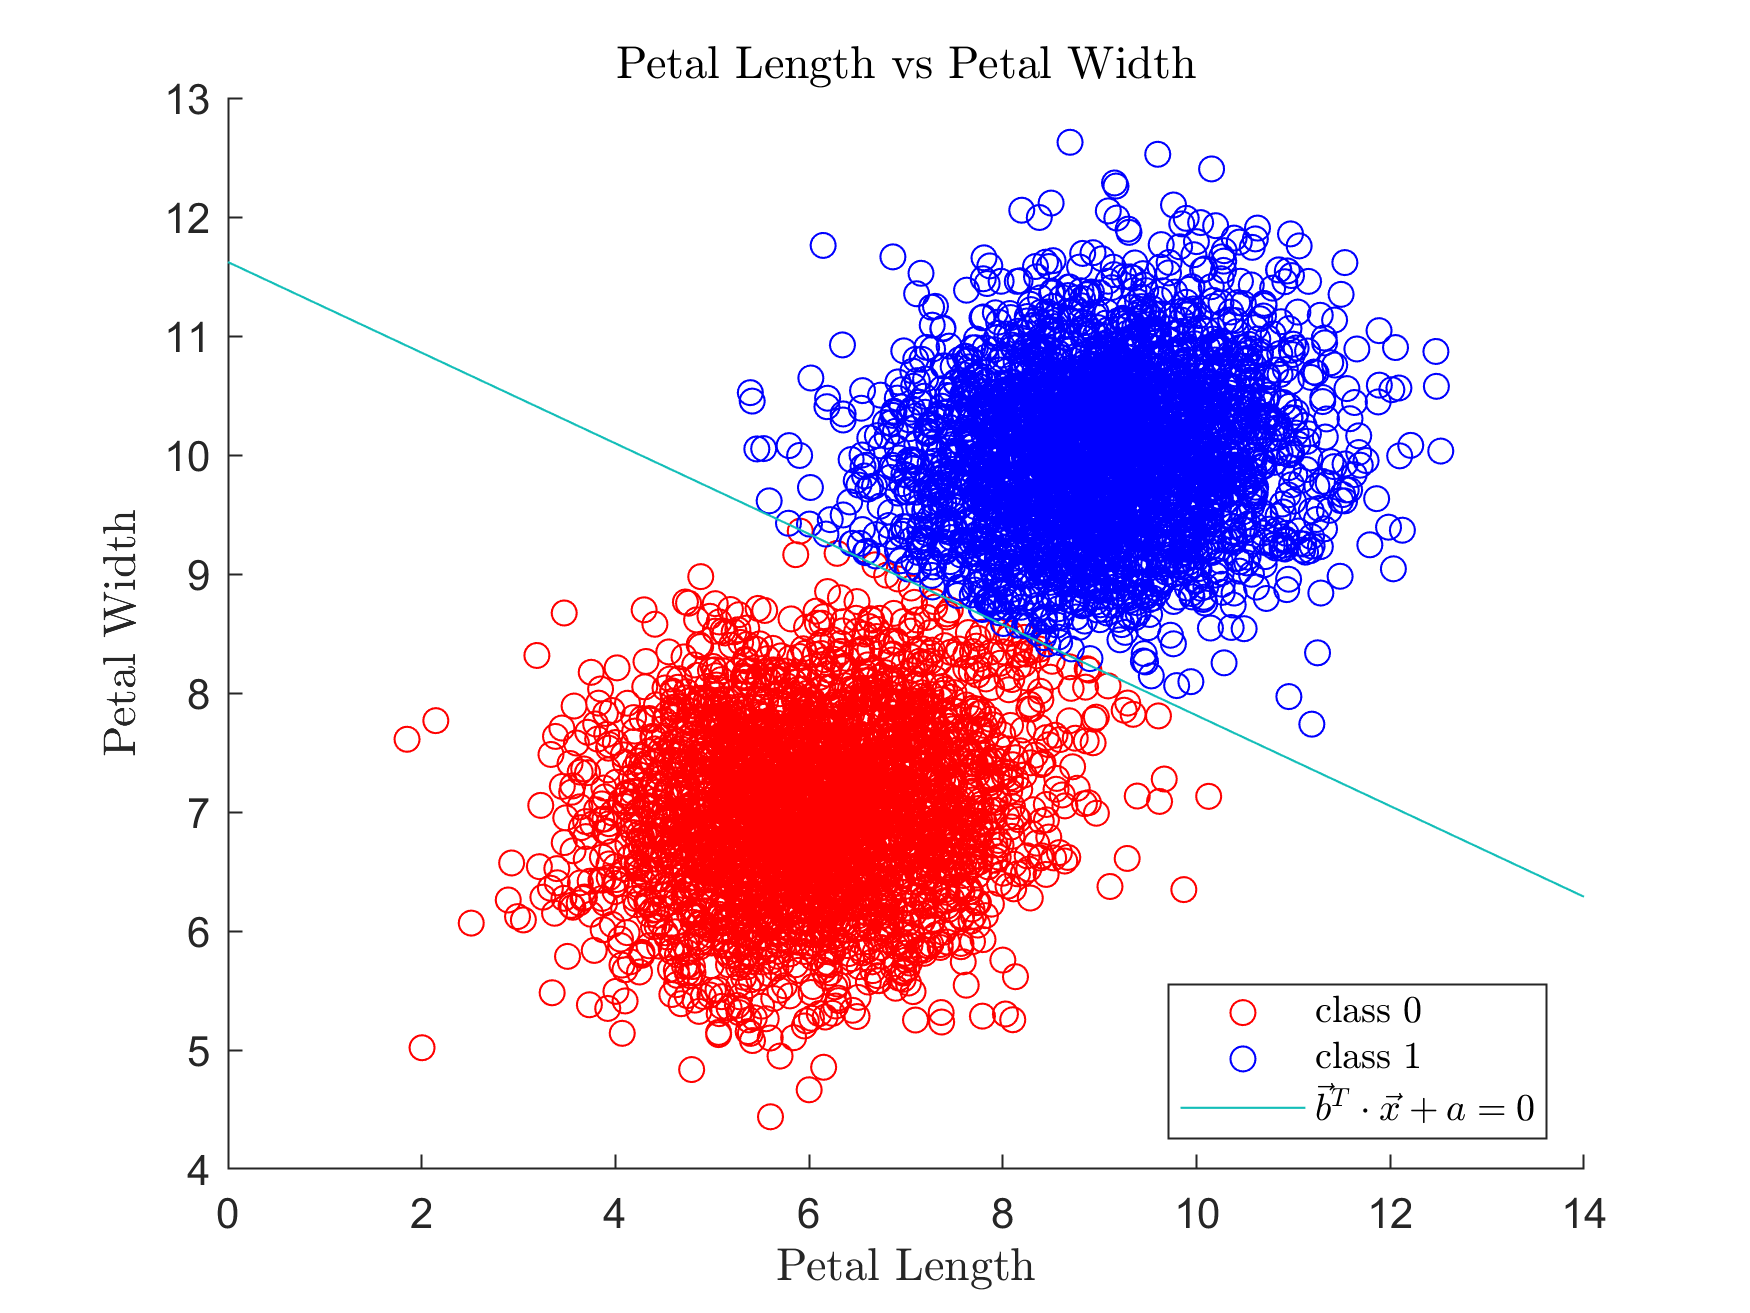
\includegraphics{03_d_scatter}
	\caption{Scatter plot and contour line of two classes from a sample with the same covariance and based on the linear inequality with $p=0.05$. Based on the samples, 50.85\% are classified as class 0. Also, the change in $p$ shifted the contour line towards the samples categorized as class 1. The result is expected given that the probability of a sample to be categorized as class 0, as opposed to 1, is higher.} 
	\label{fig:contour for p=0.05}
\end{figure}

\subsection{Quadratic Inequality}

\begin{align}
	P(y=0|\vec{x}) & \geq P(y=1|\vec{x})
	\\
	\frac{P(\vec{x}|y=0)P(y=0)}{P(\vec{x})} & \geq \frac{P(\vec{x}|y=1)P(y=1)}{P(\vec{x})} & \text{by Bayes' Rule}
	\\
	P(\vec{x}|y=0)P(y=0) & \geq P(\vec{x}|y=1)P(y=1)
	\\
	(1-p)P(\vec{x}|y=0) & \geq (p)P(\vec{x}|y=1) & \text{since }
	y=
		\begin{cases}
			1	& \text{w.p. } p
			\\
			0	& \text{w.p. } 1-p
		\end{cases}
	\\
	(1-p)f_{X,y=0}(\vec{x}) & \geq (p)f_{X,y=1}(\vec{x})
\end{align}

\begin{align}
	(1-p)f_{X,y=0}(\vec{x}) &\geq (p)f_{X,y=1}(\vec{x})
	\\
	\frac{\frac{1-p}{p}\text{exp}(\vec{x}^T\Sigma_0^{-1}\vec{x}-2\mu_0^T\Sigma_0^{-1}\vec{x}+\mu_0^T\Sigma_0^{-1}\mu_0)}{(2\pi)^{\frac{n}{2}}|\sum|^\frac{1}{2}}
	& \geq
	\frac{\text{exp}(\vec{x}^T\Sigma_1^{-1}\vec{x}-2\mu_1^T\Sigma_1^{-1}\vec{x}+\mu_1^T\Sigma_1^{-1}\mu_1)}{(2\pi)^{\frac{n}{2}}|\sum|^\frac{1}{2}}
	\\
	\frac{\frac{1-p}{p}\text{exp}(\vec{x}^T\Sigma_0^{-1}\vec{x}-2\mu_0^T\Sigma_0^{-1}\vec{x}+\mu_0^T\Sigma_0^{-1}\mu_0)}{|\sum_0|^\frac{1}{2}}
	& \geq
	\frac{\text{exp}(\vec{x}^T\Sigma_1^{-1}\vec{x}-2\mu_1^T\Sigma_1^{-1}\vec{x}+\mu_1^T\Sigma_1^{-1}\mu_1)}{|\sum_1|^\frac{1}{2}}
\end{align}

\begin{multline}
	\frac{(1-p)}{p}|\Sigma_0|^{-\frac{1}{2}}|\Sigma_1|^\frac{1}{2}\text{exp}(\vec{x}^T(\Sigma_0^{-1}-\Sigma_1^{-1})\vec{x}
	\\	
	+2(\mu_1^T\Sigma_1^{-1}-\mu_0^T\Sigma_0^{-1})\vec{x}+\mu_0^T\Sigma_0^{-1}\mu_0-\mu_1^T\Sigma_1^{-1}\mu_1)
	\geq 1
\end{multline}

\begin{multline}
	ln[\frac{(1-p)}{p}|\Sigma_0|^{-\frac{1}{2}}|\Sigma_1|^\frac{1}{2}\text{exp}(\vec{x}^T(\Sigma_0^{-1}-\Sigma_1^{-1})\vec{x}
	\\	
	+2(\mu_1^T\Sigma_1^{-1}-\mu_0^T\Sigma_0^{-1})\vec{x}+\mu_0^T\Sigma_0^{-1}\mu_0-\mu_1^T\Sigma_1^{-1}\mu_1)]
	\geq ln(1)
\end{multline}

\begin{multline}	
	\vec{x}^T(\Sigma_0^{-1}-\Sigma_1^{-1})\vec{x}+2(\mu_1^T\Sigma_1^{-1}-\mu_0^T\Sigma_0^{-1})\vec{x}
	\\	
	+[\mu_0^T\Sigma_0^{-1}\mu_0-\mu_1^T\Sigma_1^{-1}\mu_1+ln(\frac{1-p}{p}|\Sigma_0|^{-\frac{1}{2}}|\Sigma_1|^\frac{1}{2})]
	\geq 0
\end{multline}

\subsection{Quadratic Inequality Contour}

\begin{figure}[h!]
	\centering
	\vspace{-16pt}
	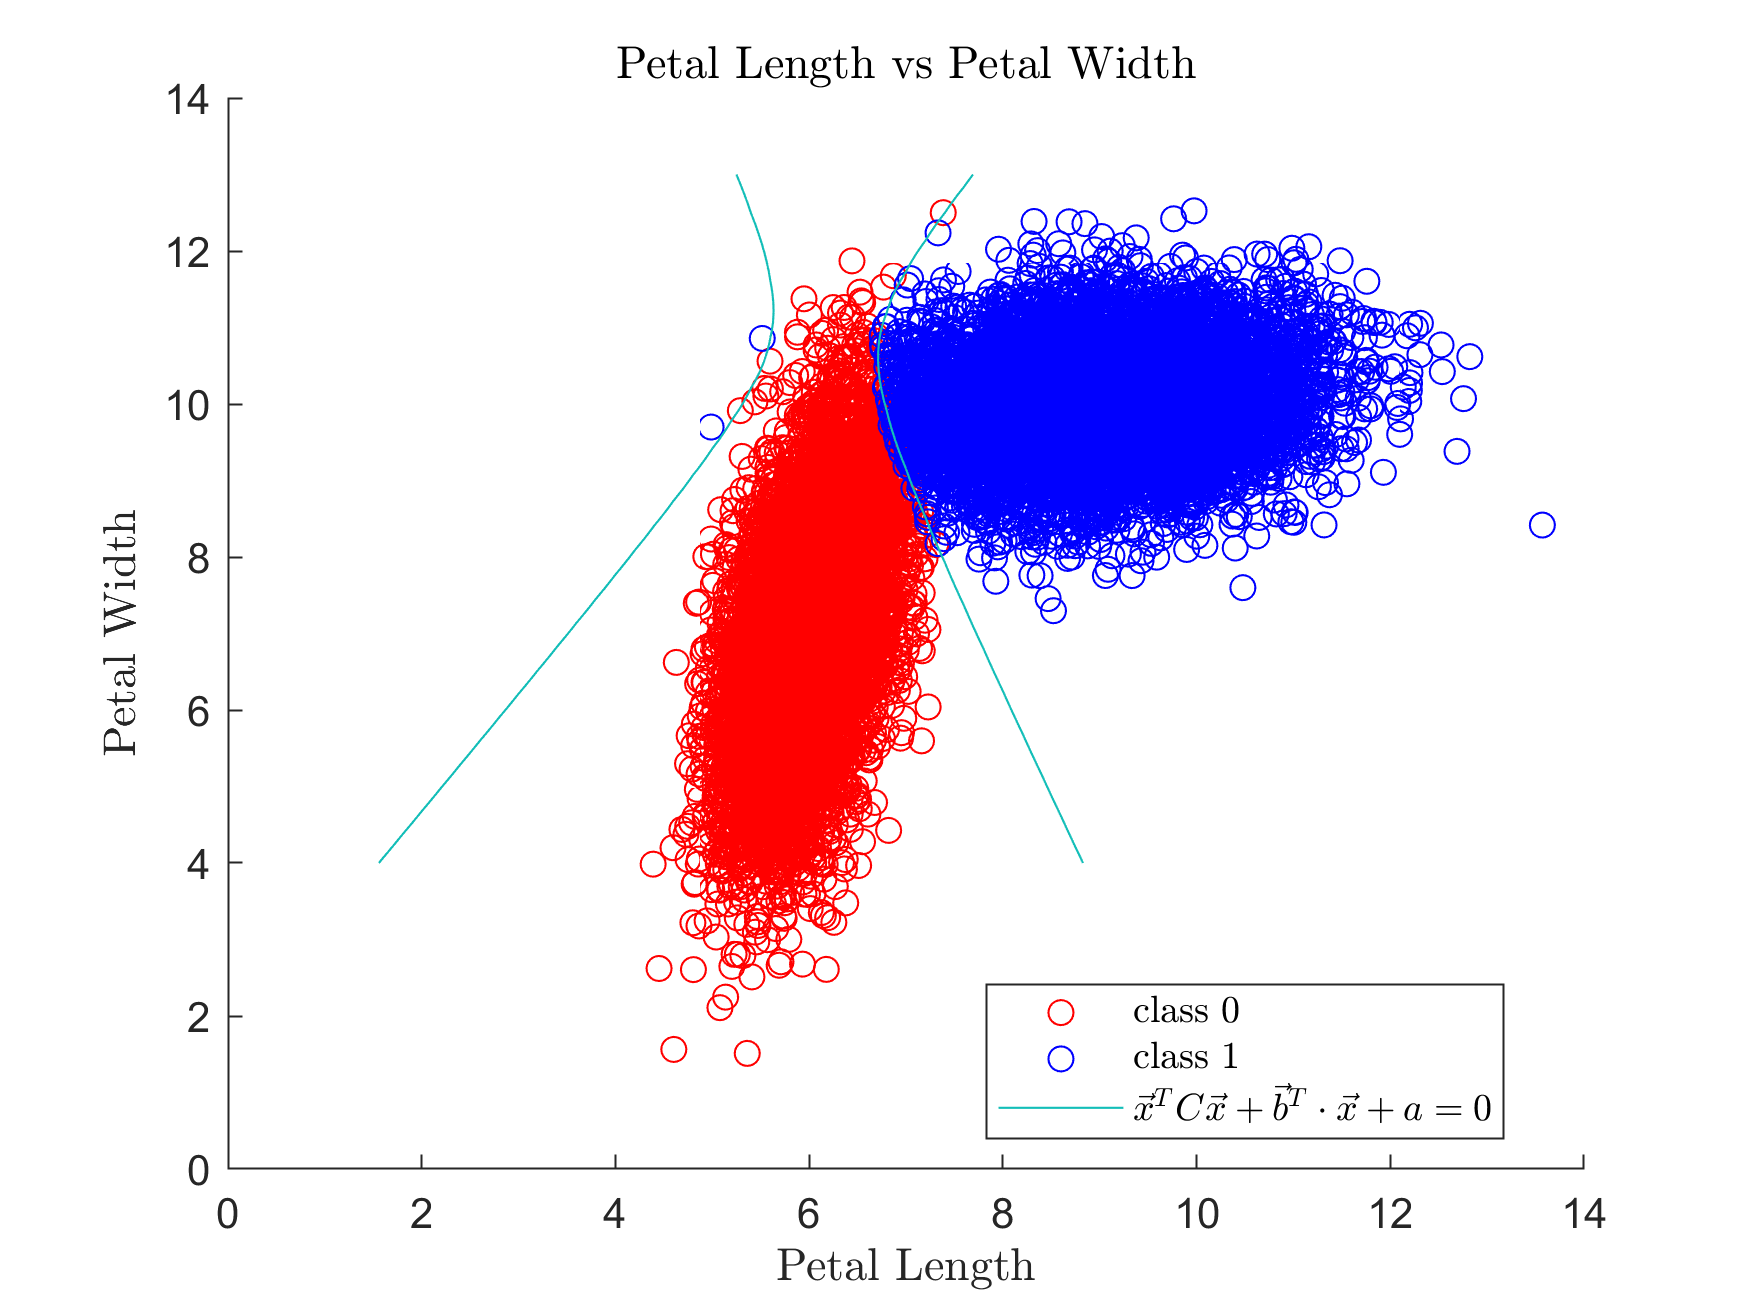
\includegraphics[scale=0.75]{03_f_scatter}
	\caption{Scatter plot and contour line of two classes from a sample with distributions that do not necessarily have the same covariances and based on the quadratic inequality with $p=0.5$. Based on the samples, 50.51\% are classified as class 0.} 
	\label{fig:quadratic contour}
\end{figure}


\lstset{language=Matlab,%
    %basicstyle=\color{red},
    breaklines=true,%
    morekeywords={matlab2tikz},
    keywordstyle=\color{blue},%
    morekeywords=[2]{1}, keywordstyle=[2]{\color{black}},
    identifierstyle=\color{black},%
    stringstyle=\color{mylilas},
    commentstyle=\color{mygreen},%
    showstringspaces=false,%without this there will be a symbol in the places where there is a space
    numbers=left,%
    numberstyle={\tiny \color{black}},% size of the numbers
    numbersep=9pt, % this defines how far the numbers are from the text
    emph=[1]{for,end,break},emphstyle=[1]\color{red}, %some words to emphasise
    %emph=[2]{word1,word2}, emphstyle=[2]{style},    
}

\section{Appendix}

\lstinputlisting{"D:/UCLA/Courses/EE 131A/Project/Code/code.m"}

\end{document}